\documentclass[lettersize,journal]{IEEEtran}
\usepackage{amsmath,amsfonts}
\usepackage{algorithmic}
\usepackage{algorithm}
\usepackage{array}
\usepackage[caption=false,font={footnotesize,rm}, labelformat=simple]{subfig}
% 1. Add 'labelformat=simple' to stop the caption from adding EXTRA parentheses

% 2. Manually add parentheses to the subfigure counter itself.
%    This forces the \ref command to include them (e.g., "1(a)"),
%    and because we used 'simple' above, the caption stays as "(a)".
\renewcommand{\thesubfigure}{(\alph{subfigure})}
\usepackage{textcomp}
\usepackage{stfloats}
\usepackage{url}
\usepackage{verbatim}
\usepackage{graphicx}
\usepackage{cite}
\usepackage{cleveref}
\usepackage{multirow}
\raggedbottom
\hyphenation{op-tical net-works semi-conduc-tor IEEE-Xplore}

% Updated with editorial comments based on text dump provided

\begin{document}

\title{Design and Implementation of a Non-coupled Integrated Transformer for a Two-phase Interleaved Flyback PFC Rectifier for USB PD 3.1 Applications}

\author{Karl Raymond Dela Cruz Roque, \IEEEmembership{Student Member, IEEE}, Haruki Hirasawa, Sihoon Choi, \IEEEmembership{Member, IEEE}, Yu Yonezawa, \IEEEmembership{Member, IEEE}, Jun Imaoka, \IEEEmembership{Member, IEEE}, and Masayoshi Yamamoto, \IEEEmembership{Member, IEEE}
        % <-this % stops a space
\thanks{Manuscript received Month xx, 2xxx; revised Month xx, xxxx; accepted Month x, xxxx. (Corresponding author: Sihoon Choi).}
\thanks{K. R. D. C. Roque, S. Choi, Y. Yonezawa, J. Imaoka and M. Yamamoto are with the Institute of Materials and Systems for Sustainability, Nagoya University, Nagoya, 464-8601, Japan (e-mail: roque.karl.raymond.dela.cruz.g46@f.mail.nagoya-u.ac.jp; choi.sihoon.w4@f.mail.nagoya-u.ac.jp; yonezawa.yu.c9@f.mail.nagoya-u.ac.jp; imaoka.jun.n9@f.mail.nagoya-u.ac.jp; yamamoto.masayoshi.n5@f.mail.nagoya-u.ac.jp).}
\thanks{H. Hirasawa is with [Affiliation Needed], Japan (e-mail: ).}}

% The paper headers
\markboth{Journal of Power Electronics,~Vol.~XX, No.~X, Month~202X}%
{Roque \MakeLowercase{\textit{et al.}}: Design and Implementation of a Non-coupled Integrated Transformer}

\maketitle

\begin{abstract}
Universal serial bus power delivery (USB PD 3.1) is a widely-applied standard for electronic device charging. In 2021, USB PD 3.1 was announced with a variable output of 5 V to 48 V and a maximum output power of 240 W. A multi-phase flyback rectifier is capable of power factor correction, galvanic isolation, and wide output voltage range, and is proposed as an alternative topology for USB PD. However, the number of magnetic components increases with the number of phases, which can lead to lower power density. This paper proposes the design of a non-coupled integrated transformer for a two-phase interleaved flyback rectifier to reduce the size and number of magnetic components. The independent operation of the integrated transformer in two phases was verified using a 240-W two-phase interleaved flyback PFC rectifier at 100 kHz switching frequency operating at discontinuous conduction mode, both in simulation and experiment. After conducting a volume analysis through the area product method, the proposed transformer is up to 19\% smaller compared to its conventional counterpart.
\end{abstract}

\begin{IEEEkeywords}
Integrated magnetics, Transformer design, two-phase interleaved flyback rectifier, USB PD 3.1, PFC, Core volume analysis.
\end{IEEEkeywords}

\section{Introduction}
\IEEEPARstart{U}{niversal} serial bus power delivery (USB PD) is a technology used for convenient, portable, fast charging in electronic devices. The latest standard, USB PD 3.1, was announced in 2021, with the maximum power supplied being up to 240 W, allowing for higher power applications \cite{ref1}. Adapters for USB PD 3.1 must be capable of power factor correction (PFC) for supporting 75 W and above, be equipped with galvanic isolation for user safety, and be capable of providing an output voltage of 5 V to 48 V \cite{ref2}.

A flyback rectifier has been widely used for commercial adapters due to its simple configuration, easy PFC control, and wide output voltage range. Improved configurations of flyback rectifiers such as active clamp flyback converters \cite{ref6, ref7} and bridgeless flyback rectifiers have also been proposed for higher converter efficiency \cite{ref8, ref9, ref10, ref11}. However, they are generally more practical for lower power applications due to the inherent high current stress on the switches by these topologies.

Several power supply configurations for USB PD 3.1 have been proposed to meet the requirements. One example is a combination of a PFC rectifier, an LLC converter, and a buck converter as shown in Fig. \ref{fig:1a} \cite{ref3, ref4}. The LLC converter is not suitable for wide output voltage and requires a buck converter in its subsequent stage, though it realizes high power density. Three stages of power conversion also lead to many circuit components and therefore high cost. An asymmetrical half bridge (AHB) flyback converter in the second stage of a boost PFC circuit was introduced as shown in \ref{fig:1b} \cite{ref5}. The AHB allows for zero-voltage switching (ZVS) by the application of resonant capacitors in series placed on the primary side of the transformer. However, the design of this circuit is complicated especially because the resonant design must take into account the leakage inductance of the transformer.

\begin{figure}[htbp]
\centering
% (a) Top circuit
        \subfloat[]{
        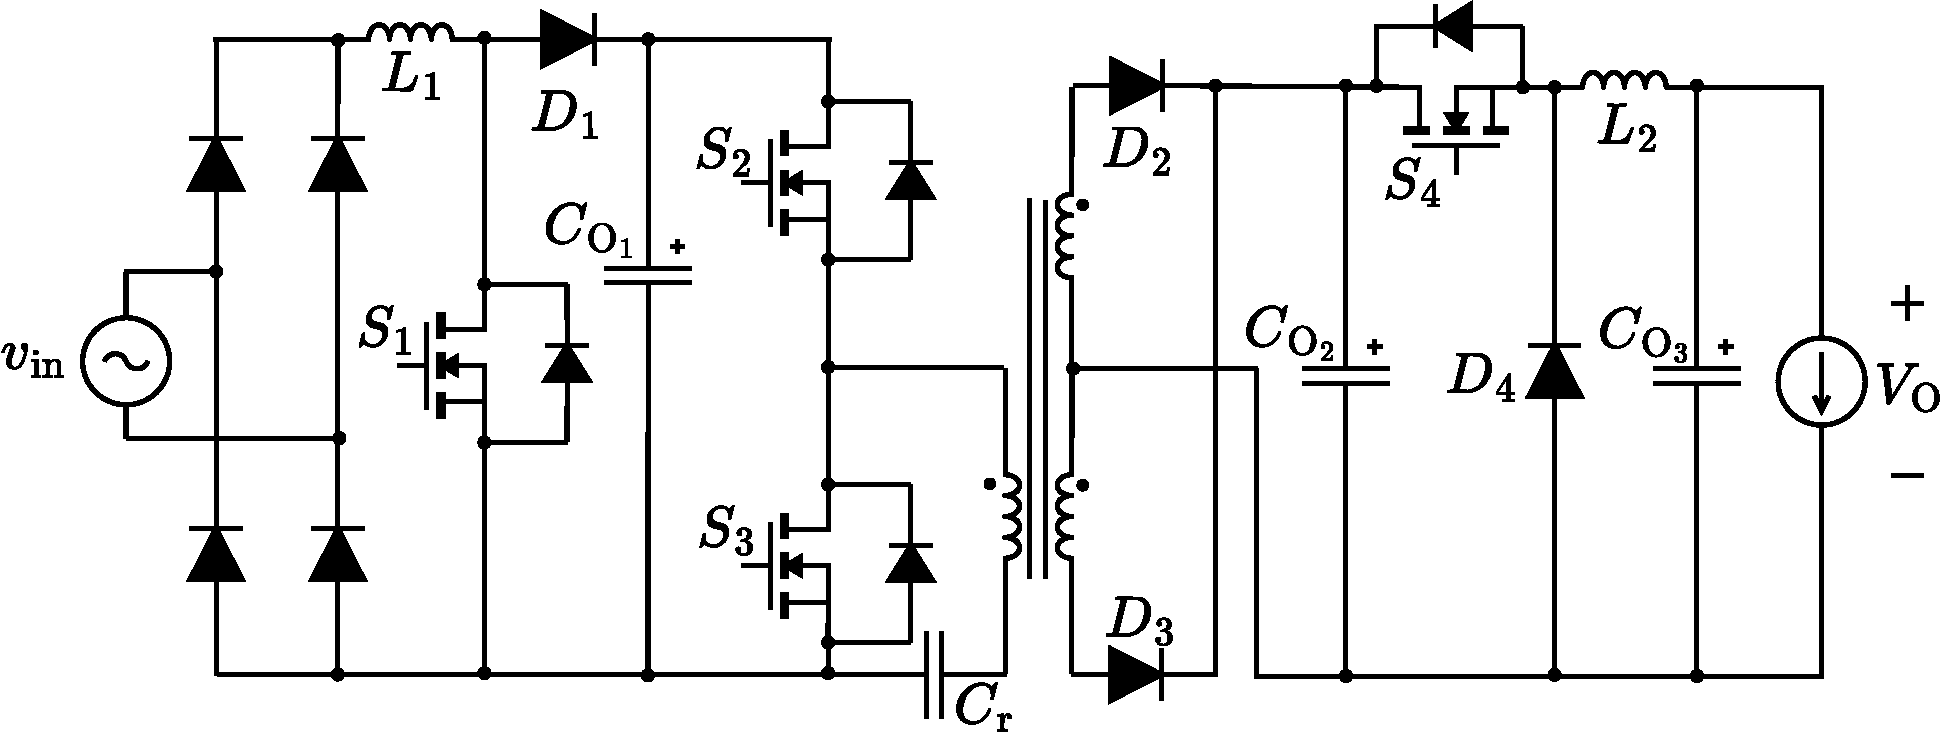
\includegraphics[width=\columnwidth]{Figures_v2/Fig1a.pdf} % Make sure this file exists
        \label{fig:1a}
        }
        \\ % This double backslash forces the next image to the line below (vertical stack)
        % (b) Middle circuit
        \subfloat[]{
        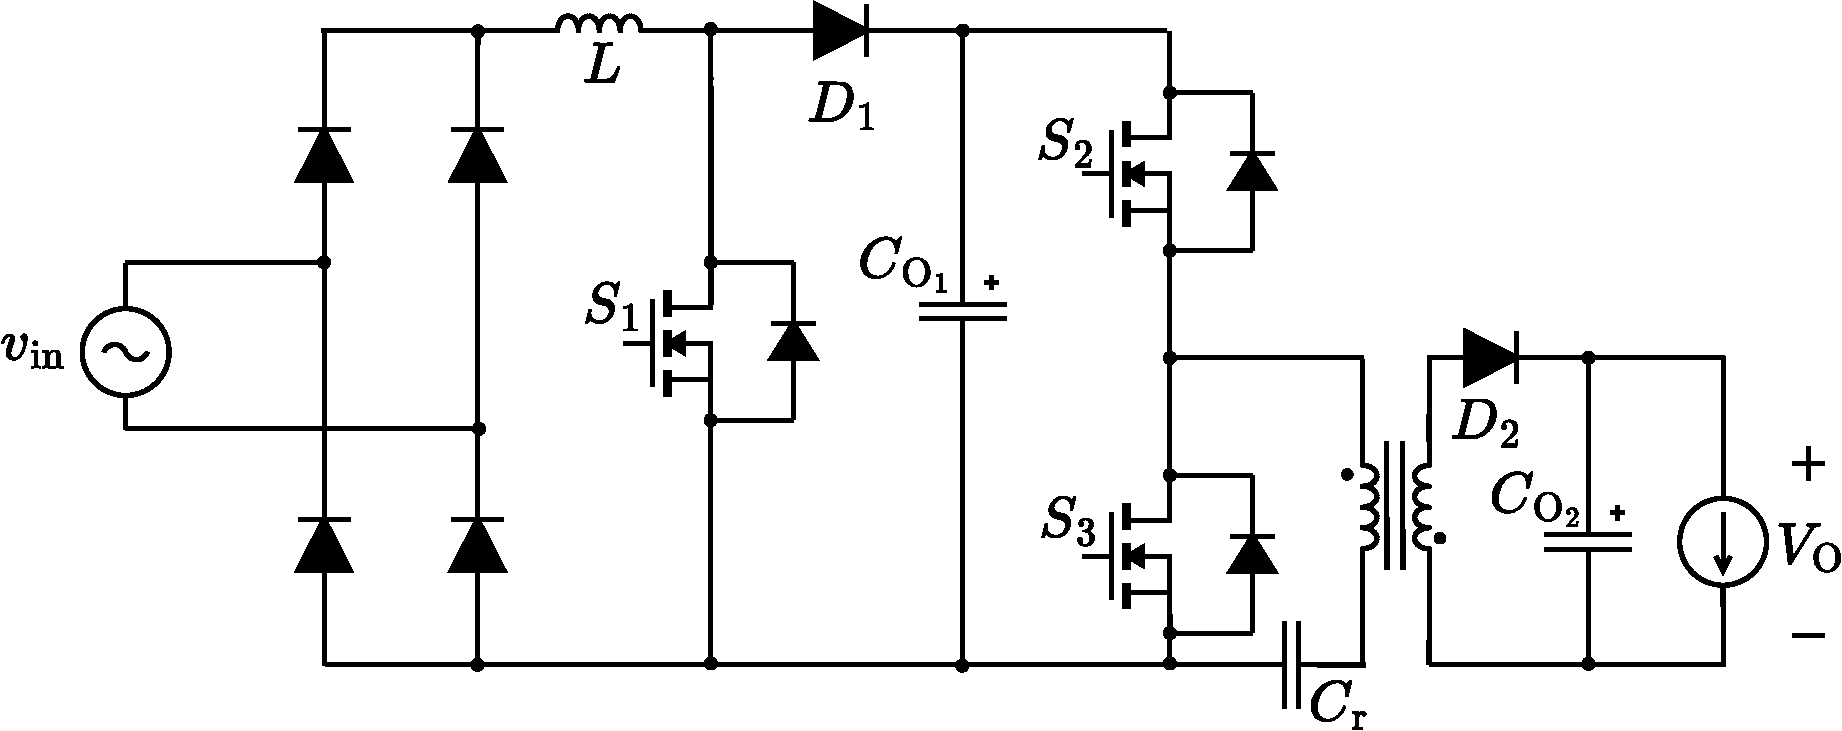
\includegraphics[width=\columnwidth]{Figures_v2/Fig1b.pdf}
        \label{fig:1b}
        }
        \\ % Line break
        % (c) Bottom circuit
        \subfloat[]{
        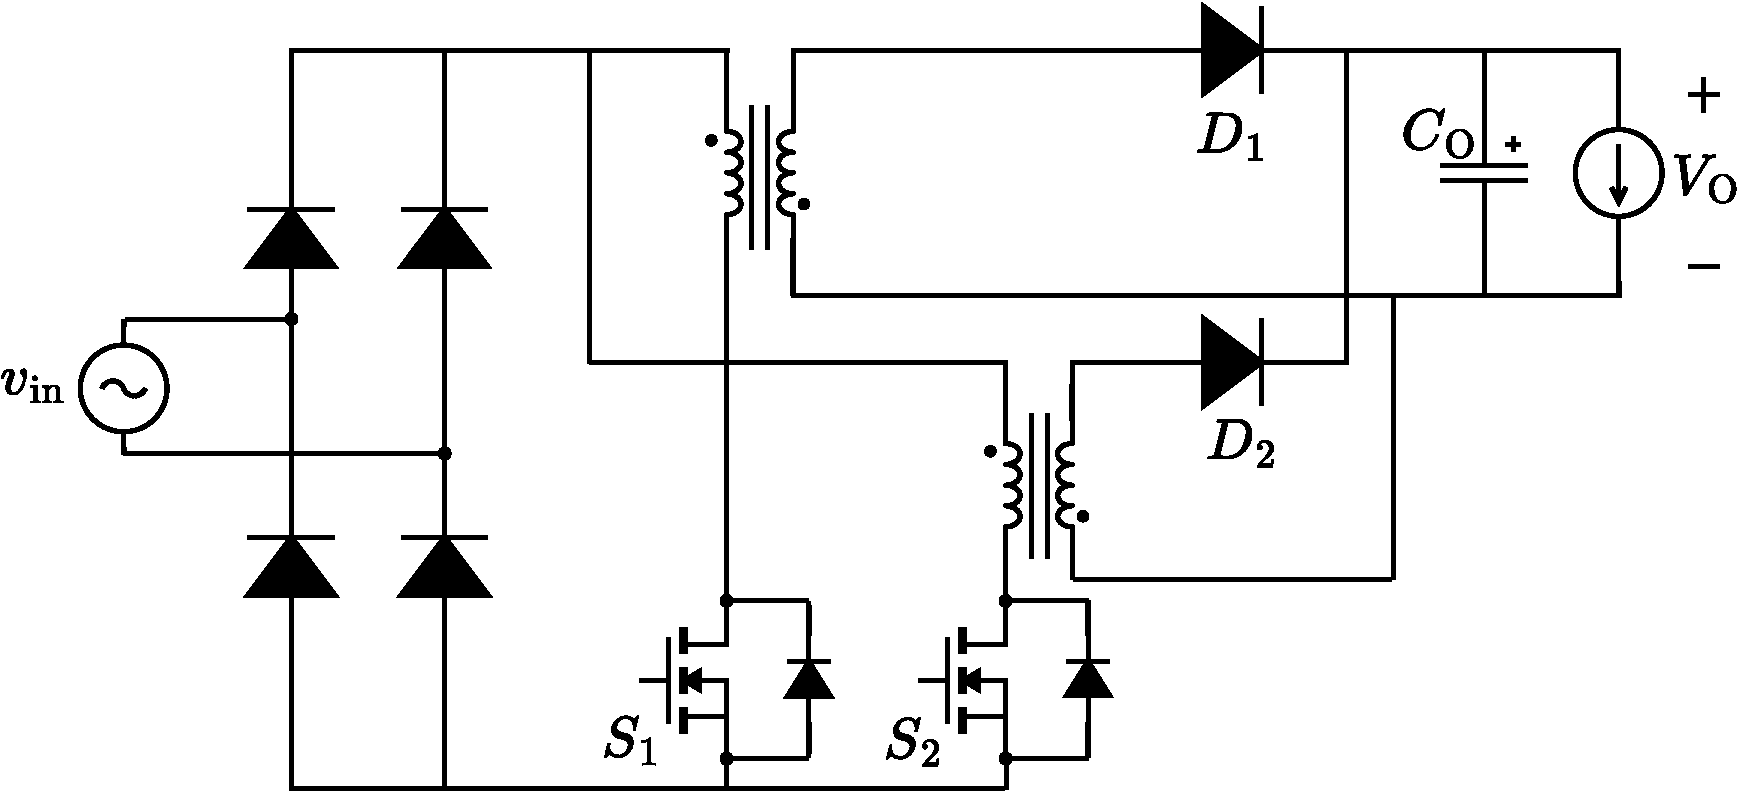
\includegraphics[width=\columnwidth]{Figures_v2/Fig1c.pdf}
        \label{fig:1c}
        }
        \caption{Power supply configurations proposed for PD 3.1 applications: (a) PFC boost, LLC, and buck converter combination in \cite{ref3,ref4}, (b) PFC boost with AHB flyback \cite{ref1}, (c) two-phase interleaved flyback PFC rectifier.}
        \label{fig:configurations}
\end{figure}

Interleaving rectifiers have also been considered to increase the maximum output power. Two-phase interleaving allows half of the total power to be supplied in each phase, therefore reducing the possible stress on the circuit elements \cite{ref12}. The topology is shown in Fig. \ref{fig:1c}, where the two phases are parallel in the input and output side. The source nodes of switches $S_1$ and $S_2$ are common, and only one power supply is required for gate drive circuits. A common cathode package can be used for diodes $D_1$ and $D_2$. Fewer components can configure the circuit though two transformers are required. However, adopting two transformers may dilute the advantage of the flyback rectifier.

Integrated magnetics have been widely utilized to minimize component size and improve power density. The transformer in \cite{ref15} features one set of primary and secondary windings placed on each of the outer legs of a three-legged core. This arrangement does not allow for flux cancellation in the center leg and is designed such that both transformers operate simultaneously. While this structure may help reduce input capacitor loss by distributing the ripple current, it requires precise tuning of the input current ripple and coupling, adding complexity to the design. The transformer in \cite{ref16} adopts a similar physical layout as in \cite{ref15}, but with the windings arranged to enable flux cancellation in the center leg. Coupling between the windings allows for a reduction in input current ripple; however, the design becomes more complex, since the magnetic coupling affects zero-voltage switching (ZVS) and active clamping. The transformer in \cite{ref17} also uses a similar configuration, but with inversely coupled secondary windings. In this case, careful design of the secondary-side coupling is required to meet specific output current ripple requirements, and the inverse coupling may introduce unwanted circulating currents or EMI if not properly managed. The transformer in \cite{ref18} adds an inductor winding on the center leg, in addition to the transformers on the outer legs, to further control output current ripple. However, this increases the core's magnetic complexity and can make magnetic design and analysis more challenging. A detailed comparison of these integrated magnetics structures is provided in Table \ref{tab:transformer_comparison}.
\begin{table*}[htbp]
\centering
% This command sets the font size for the entire table environment
\footnotesize 
\caption{Comparison of Integrated Magnetics Techniques with the Proposed Transformer}
\label{tab:transformer_comparison}

% Columns defined as 'm' (middle vertical align) but with \raggedright (left horizontal align)
% We define a custom column type 'L' for convenience: Left aligned, Middle vertical
\newcolumntype{L}[1]{>{\raggedright\arraybackslash}m{#1}}
% We define a custom column type 'C' for the images/citations: Centered, Middle vertical
\newcolumntype{C}[1]{>{\centering\arraybackslash}m{#1}}

\setlength{\tabcolsep}{2pt}
\begin{tabular}{|L{1.8cm}|L{2.8cm}|L{2.8cm}|L{2.8cm}|L{2.8cm}|L{2.8cm}|}
\hline

% Row 1: Images (Using C column alignment locally or \centering)
% Note: We use \multicolumn to override the 'L' alignment for images if desired, 
% or simply use \centering inside the cell.
 & 
 \centering\arraybackslash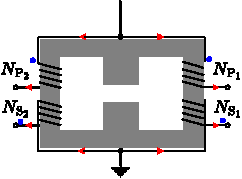
\includegraphics[width=\linewidth]{Figures_v2/Table15.pdf} & 
 \centering\arraybackslash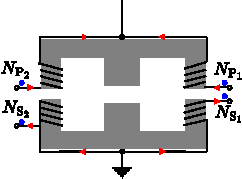
\includegraphics[width=\linewidth]{Figures_v2/Table16.pdf} & 
 \centering\arraybackslash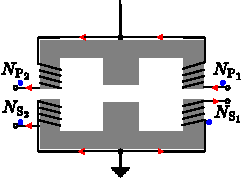
\includegraphics[width=\linewidth]{Figures_v2/Table17.pdf} & 
 \centering\arraybackslash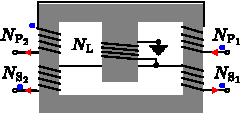
\includegraphics[width=\linewidth]{Figures_v2/Table18.pdf} & 
 \centering\arraybackslash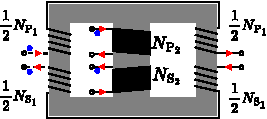
\includegraphics[width=\linewidth]{Figures_v2/Tableprop.pdf} \\ 
\hline

% Row 2: Citations (Centered looks better for these, so we add \centering)
\textbf{Transformer} & 
\centering\arraybackslash [15] & 
\centering\arraybackslash [16] & 
\centering\arraybackslash [17] & 
\centering\arraybackslash [18] & 
\centering\arraybackslash \textbf{Proposed Transformer} \\ 
\hline

% Row 3: Topology (Left aligned - default for our L columns)
Circuit Topology & 
Two-phase Interleaved Flyback & 
Two-phase Interleaved Forward & 
Two-phase Interleaved Flyback & 
Full-wave converter & 
\textbf{Two-phase Interleaved Flyback} \\ 
\hline

% Row 4: Operation
Operation & 
CCM, step-up & 
CCM, step-down & 
CCM, step-down & 
CCM, step-down & 
\textbf{DCM, step-down} \\ 
\hline

% Row 5: Config
Transformer Configuration & 
Series-input, Parallel-output & 
Series-input, Parallel-output & 
Series-input, Parallel-output & 
Parallel-input and output & 
\textbf{Parallel-input and output} \\ 
\hline

% Row 6: Coupling
Coupling between Transformers & 
Yes & 
Yes & 
Yes (inverse coupling) & 
Yes & 
\textbf{No} \\ 
\hline

% Row 7: Flux Cancellation
Flux Cancellation in Middle Leg & 
No & 
Yes & 
No & 
- & 
\textbf{Yes} \\ 
\hline

% Row 8: Air Gap
Air Gap & 
Center leg & 
Outer and Center Legs & 
Outer and Center Legs & 
- & 
\textbf{Outer and Center Legs} \\ 
\hline

% Row 9: Features
Feature of Circuit with Transformer & 
Less input capacitor losses due to reduction of input current ripple. & 
Input current ripple reduction & 
Output current ripple reduction & 
Output current ripple controllable & 
\textbf{2 phase independent operation, 1 phase drive possible.} \\ 
\hline

% Row 10: Design Method
Design Method & 
Uses primary side current ripple and peak flux (affected by coupling coefficient) & 
Transformer designed with accordance to implementation of ZVS and Active Clamping. & 
Uses primary side current ripple, saturation magnetic flux density, and coupling coefficient & 
Uses primary side current ripple, and saturation magnetic flux density & 
\textbf{Uses duty cycle and saturation magnetic flux density} \\ 
\hline

\end{tabular}
\end{table*}

This paper proposes a non-coupled integrated transformer for a two-phase interleaved flyback rectifier as shown in Fig. \ref{fig:2a}. The proposed winding structure is shown in Fig. \ref{fig:2b} where $N_{12}$ is the number of turns between terminals 1 and 2. Half of $N_{12}$ and $N_{34}$ are wound at each outer leg with opposite polarity, so as to allow for flux cancellation at the center leg. On the other hand, $N_{56}$ and $N_{78}$ are also wound with opposite polarity on the center leg, and allows for the transformer $N_{12}$ and $N_{34}$ to not operate during its operation. Therefore, the proposed winding structure employs zero coupling coefficient between the two transformers $N_{12}-N_{34}$ and $N_{56}-N_{78}$.

\begin{figure}[t]
\centering
% (a) Top circuit
        \subfloat[]{
        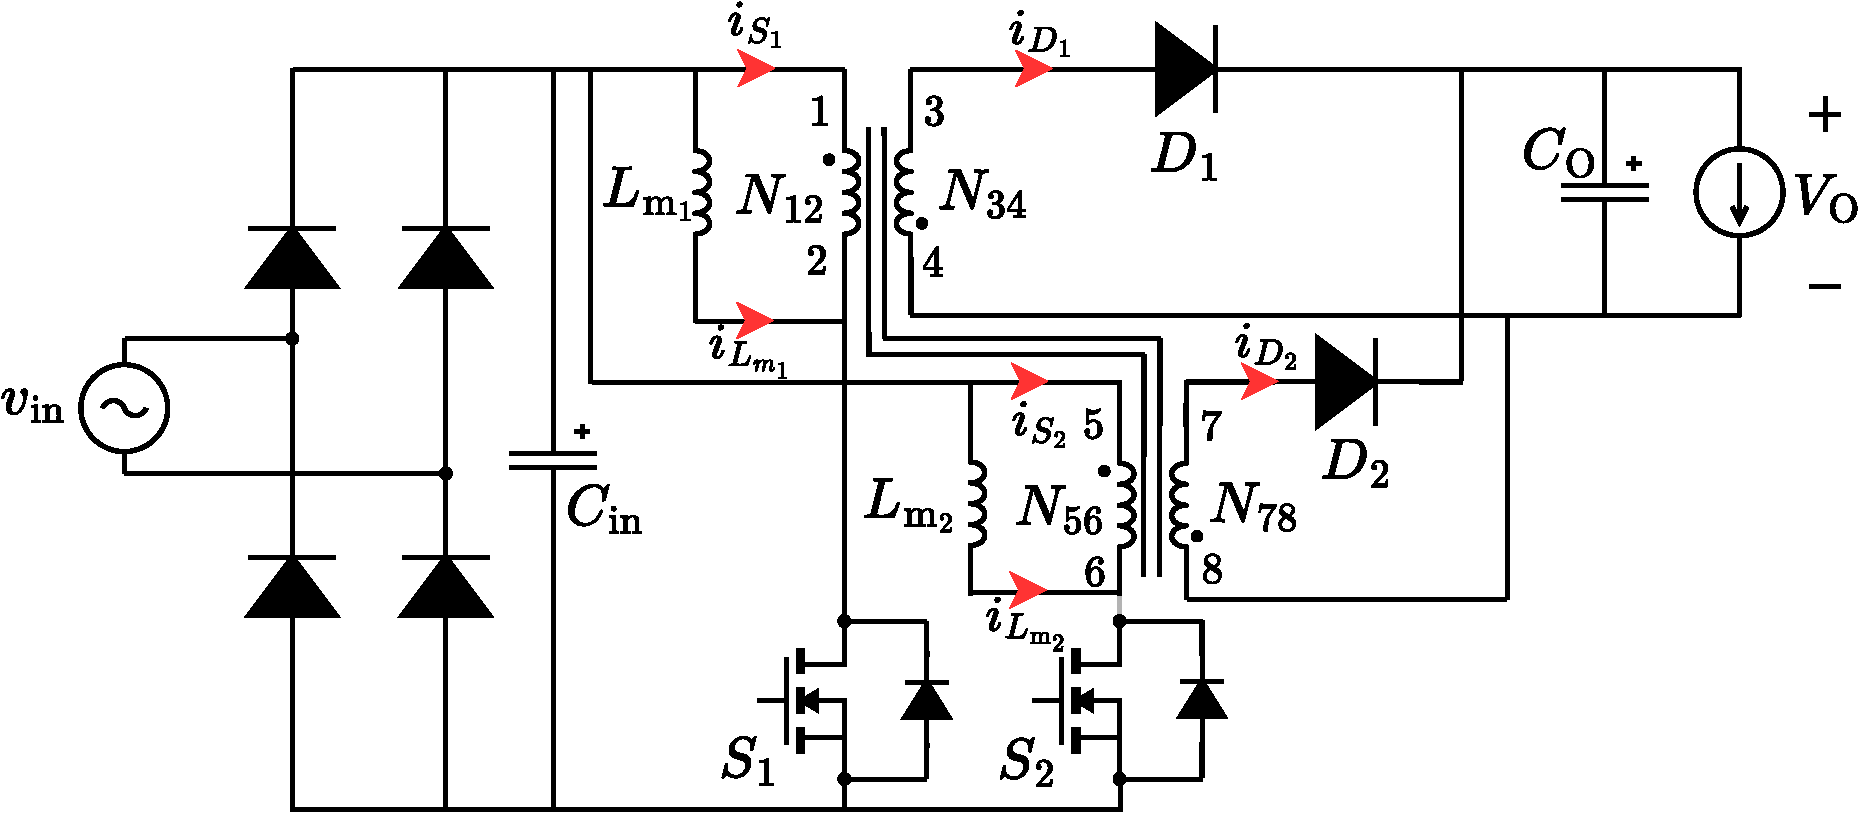
\includegraphics[width=\columnwidth]{Figures_v2/Fig2a.pdf} % Make sure this file exists
        \label{fig:2a}
        }
        \\ % This double backslash forces the next image to the line below (vertical stack)
        % (b) Middle circuit
        \subfloat[]{
        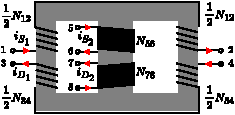
\includegraphics[width=0.6\columnwidth]{Figures_v2/Fig2b.pdf}
        \label{fig:2b}
        }
        \caption{The two-phase interleaved flyback rectifier (a), with the transformer and its winding structure in (b).}
\end{figure}

The zero-coupling coefficient between the two separate transformers simplifies implementation of rectifiers and transformer design. The operation of the rectifiers in each interleaved phase still follows that of a conventional flyback converter, preserving simplicity in control and timing. The design is also highly dependent on the duty cycle, an easily adjustable parameter in circuit design. The converter in this study aims to operate in DCM in order to allow for easier implementation of PFC and to conform to the standards of USB PD 3.1. It also realizes independent phase operation, allowing the circuit to function in one-phase mode if desired, thereby enhancing flexibility in circuit operation.

The rest of this paper is organized as follows: Section II presents an operational analysis of a two-phase interleaved flyback rectifier with the integrated transformer, along with its design method. Section III describes the size reduction effect of the transformer. Sections IV and V discuss the results of the simulation and experimental verification respectively, and Section VI presents the conclusions of this paper.

\section{Design Method of the Proposed Transformer}

\subsection{Operation Analysis of the Converter and Transformer}
The proposed integrated transformer was designed for a two-phase interleaved flyback PFC rectifier operating in discontinuous conduction mode (DCM). The switches ($S_1$, $S_2$ in Fig. \ref{fig:2a}) operate with a fixed duty cycle $D$ and a 180-degree phase shift.

Half of $N_{12}$ and $N_{34}$ are wound at each outer leg with opposite polarity. Moreover, $N_{56}$ and $N_{78}$ are also wound with opposite polarity at the center leg. The transformer utilized an EE Core with a center leg that has a cross sectional area twice its outer leg, as per commercial standard, causing $N_{12}=2N_{56}$ and $N_{34}=2N_{78}$. The magnetizing inductances for both transformers $N_{12}-N_{34}$ and $N_{56}-N_{78}$ were set to be the same. The saturation magnetic flux in each separate transformer during each phase is expected to be consistent.

The operational principle of the rectifier with the proposed transformer is illustrated in Fig. \ref{fig:operation_modes}. Additionally, Fig. \ref{fig:4} presents the key waveforms of the six distinct operation modes. The rectifier is designed with duty cycle $D \le 0.5 \frac{n V_{\mathrm{o}}}{V_{\mathrm{in}_{\mathrm{max}}}}$ with $n$ as the turns ratio, $V_{\mathrm{o}}$ as the output voltage, and $V_{\mathrm{in}_{\mathrm{max}}}$ as the peak value of the input voltage. This condition ensures the magnetizing current of one phase returns to zero before the other phase peaks. This duration is defined as the discharge time $t_{\mathrm{dis}}$ and is given in terms of circuit parameters by \eqref{eq:discharge}:

\begin{figure*}[htbp]
    \centering
    
    % --- LEFT COLUMN (Modes 1, 2, 3) ---
    % These will automatically get labels (a), (b), (c)
    \begin{minipage}{0.48\textwidth}
        \centering
        
        \subfloat[\label{fig:mode_1}]{%
            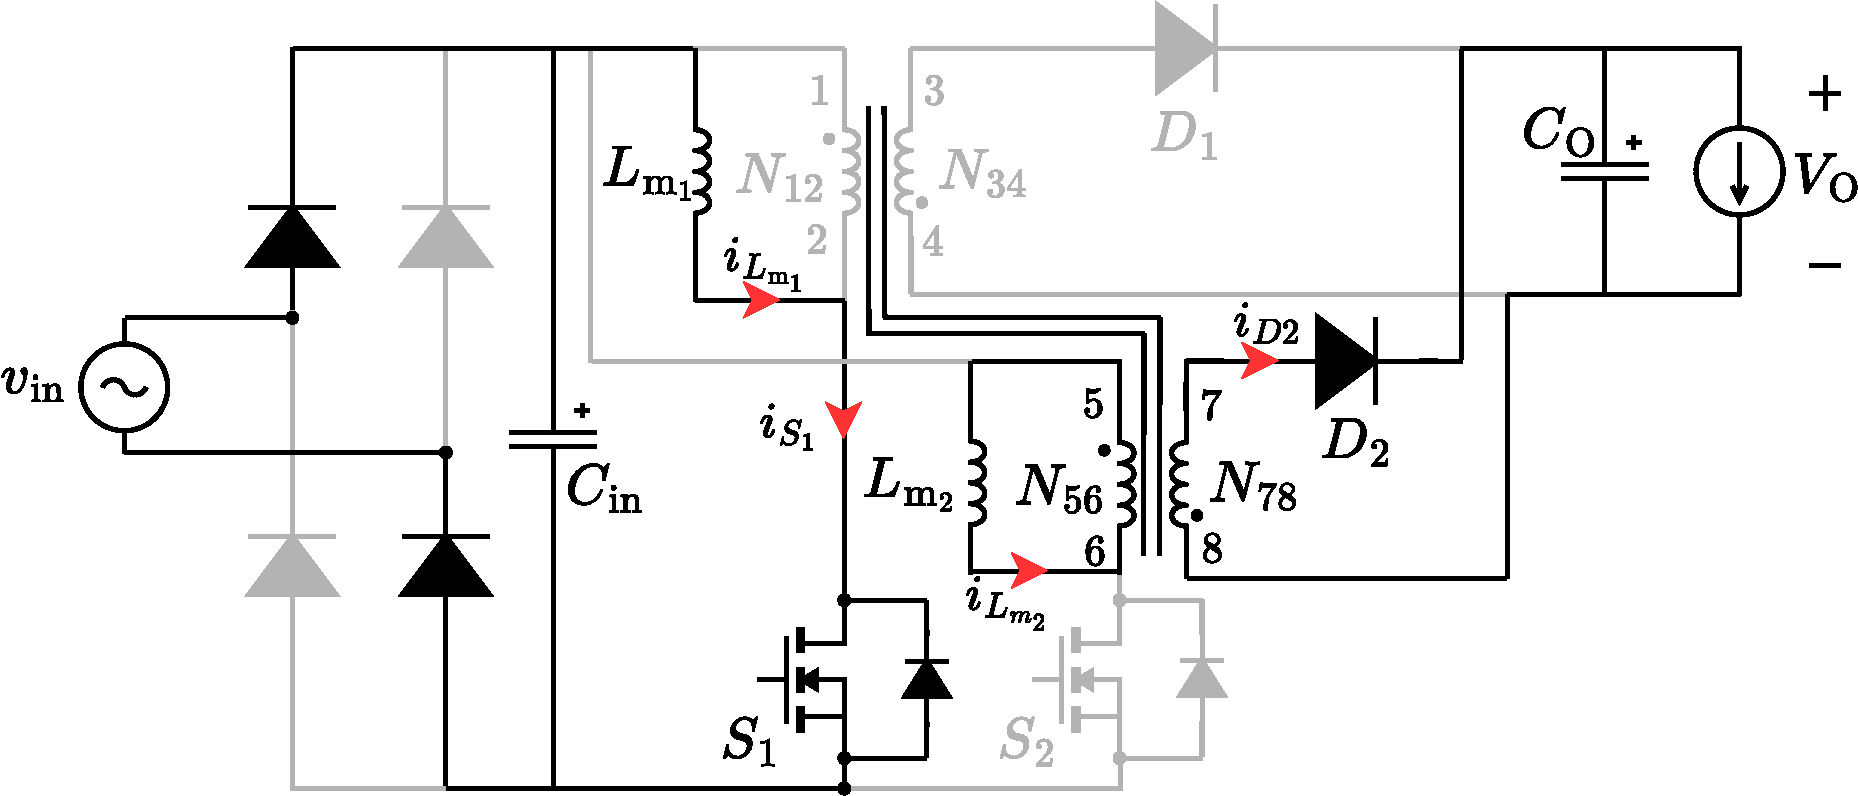
\includegraphics[width=\linewidth]{Figures_v2/Fig3a.pdf}%
        }
        
        \vspace{10pt} % Spacing between Mode 1 and 2
        
        \subfloat[\label{fig:mode_2}]{%
            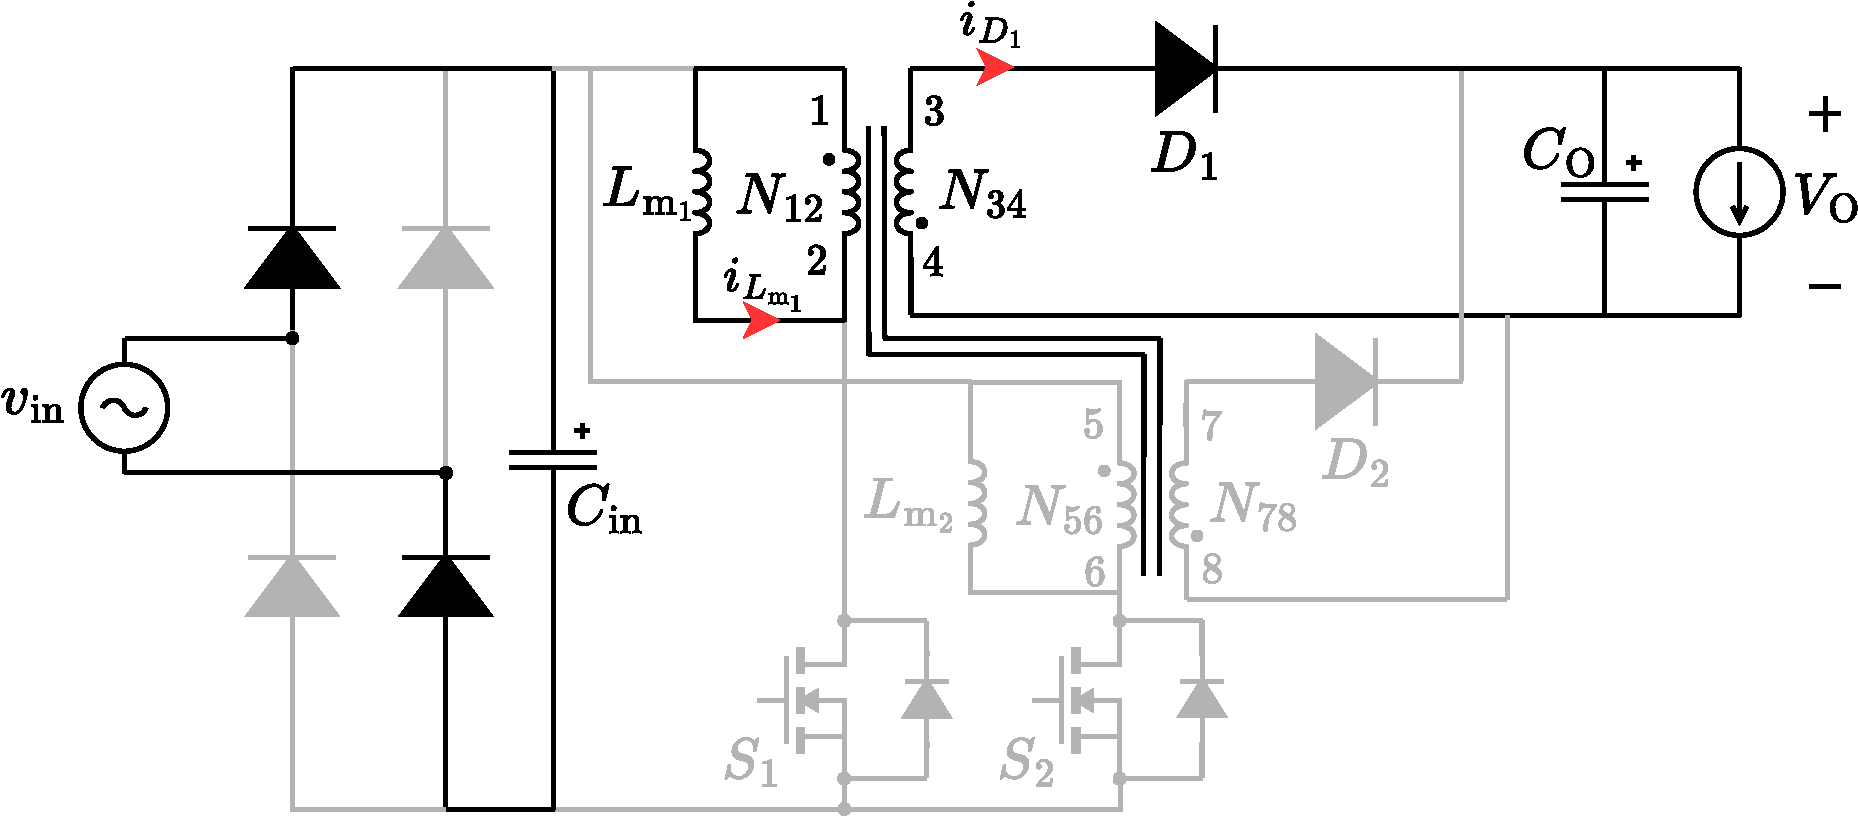
\includegraphics[width=\linewidth]{Figures_v2/Fig3c.pdf}%
        }
        
        \vspace{10pt} % Spacing between Mode 2 and 3
        
        \subfloat[\label{fig:mode_3}]{%
            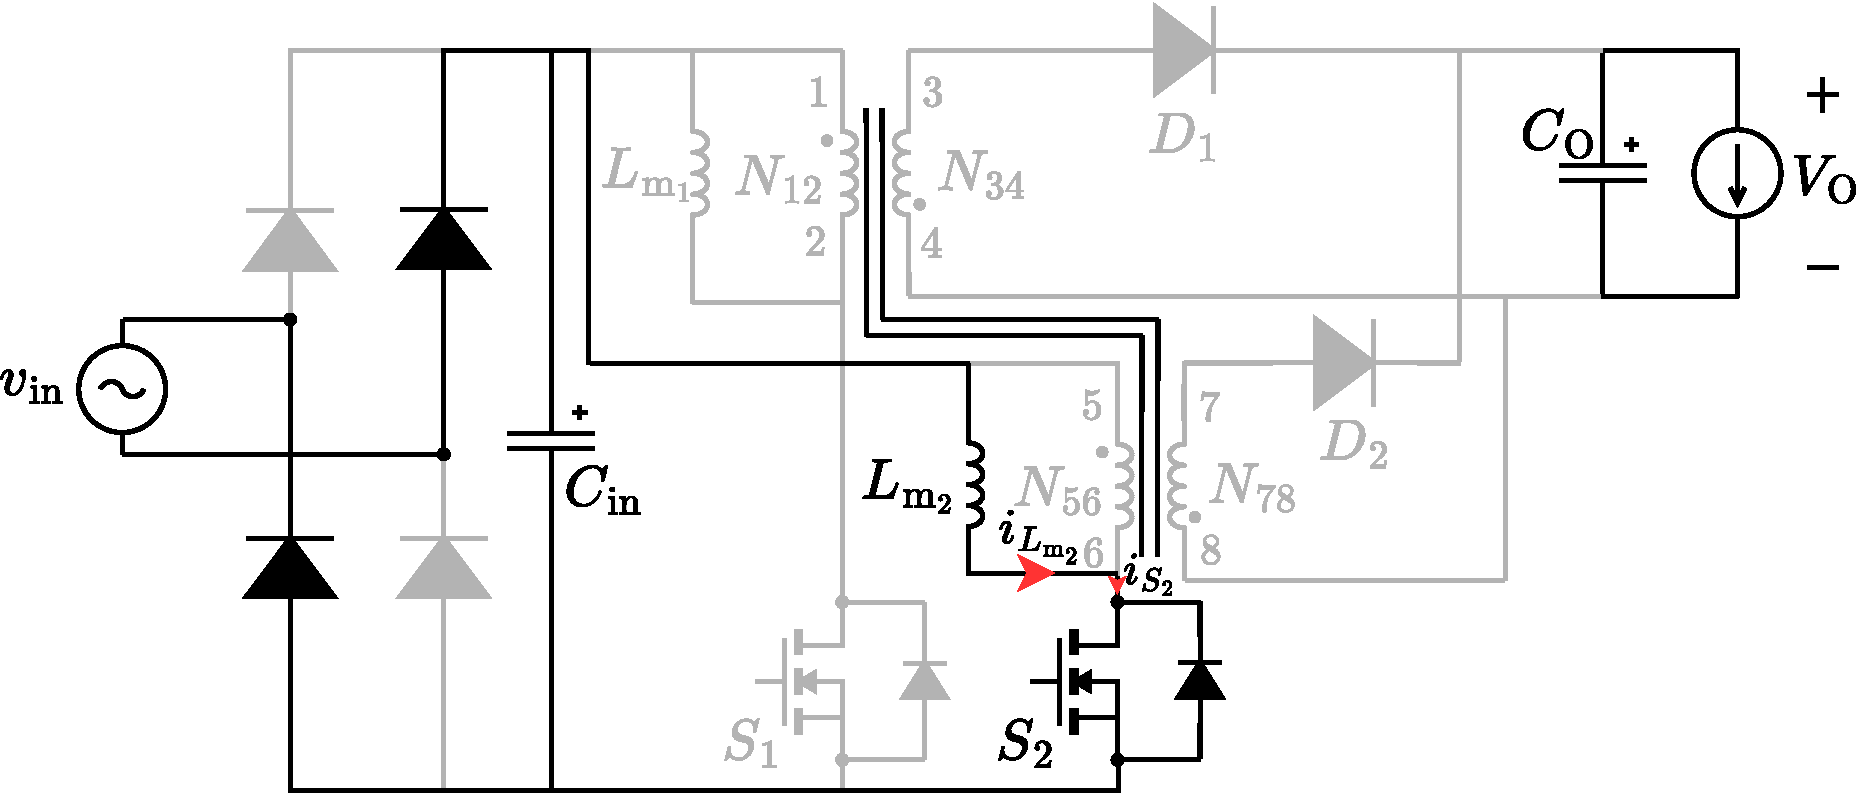
\includegraphics[width=\linewidth]{Figures_v2/Fig3e.pdf}%
        }
    \end{minipage}
    \hfill % Horizontal space between the two columns
    % --- RIGHT COLUMN (Modes 4, 5, 6) ---
    % These will automatically get labels (d), (e), (f)
    \begin{minipage}{0.48\textwidth}
        \centering
        
        \subfloat[\label{fig:mode_4}]{%
            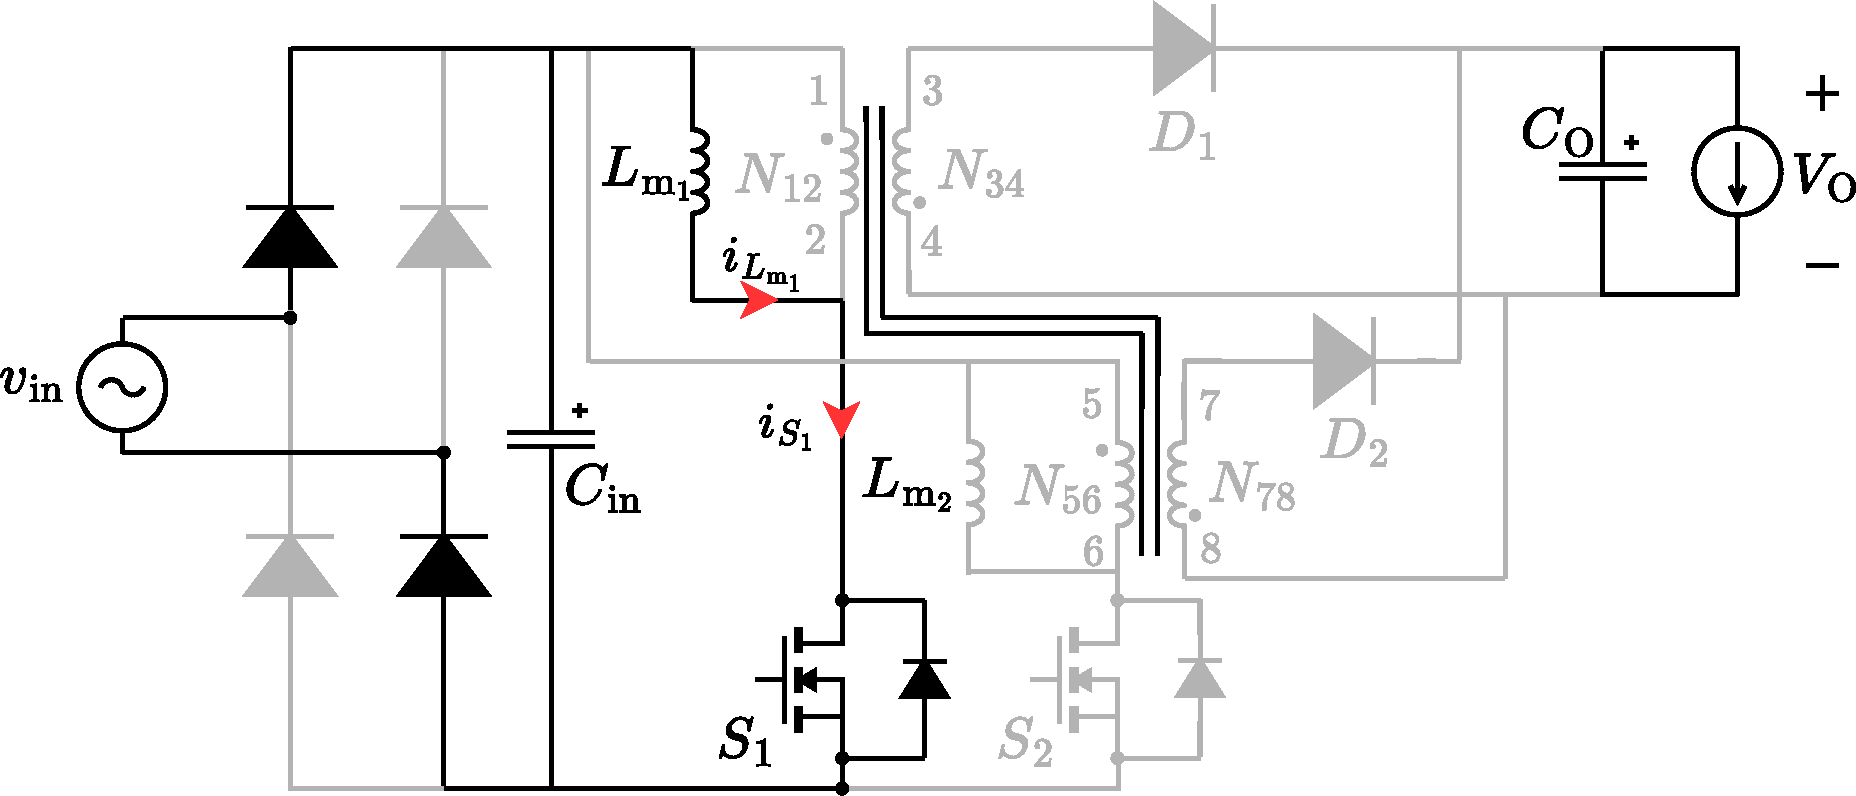
\includegraphics[width=\linewidth]{Figures_v2/Fig3b.pdf}%
        }
        
        \vspace{10pt} 
        
        \subfloat[\label{fig:mode_5}]{%
            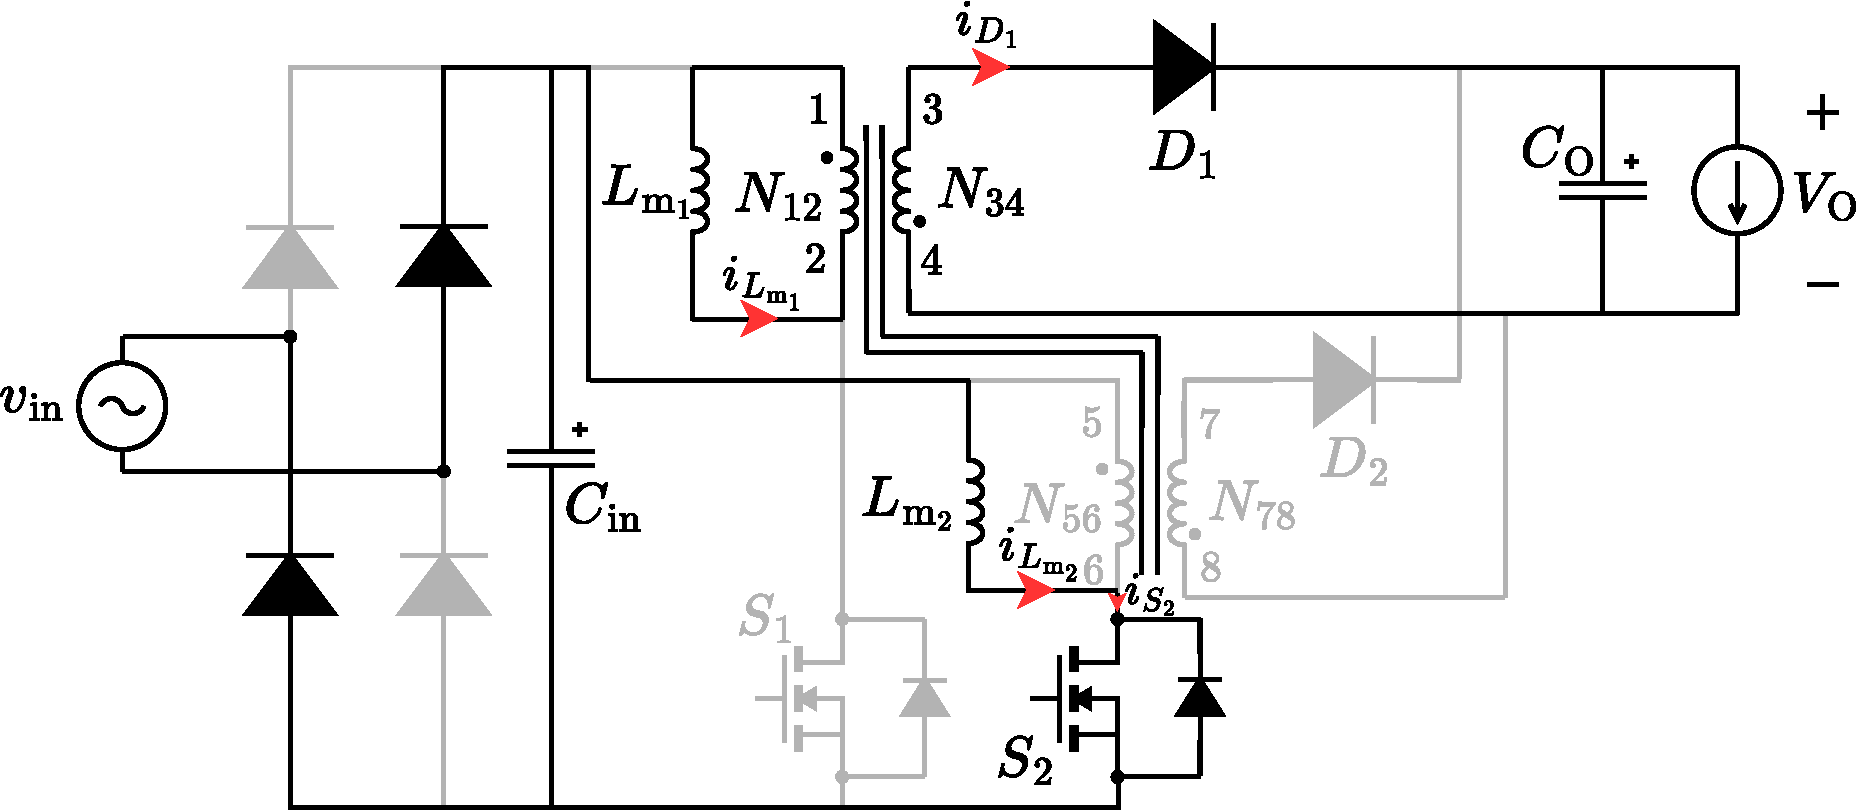
\includegraphics[width=\linewidth]{Figures_v2/Fig3d.pdf}%
        }
        
        \vspace{10pt} 
        
        \subfloat[\label{fig:mode_6}]{%
            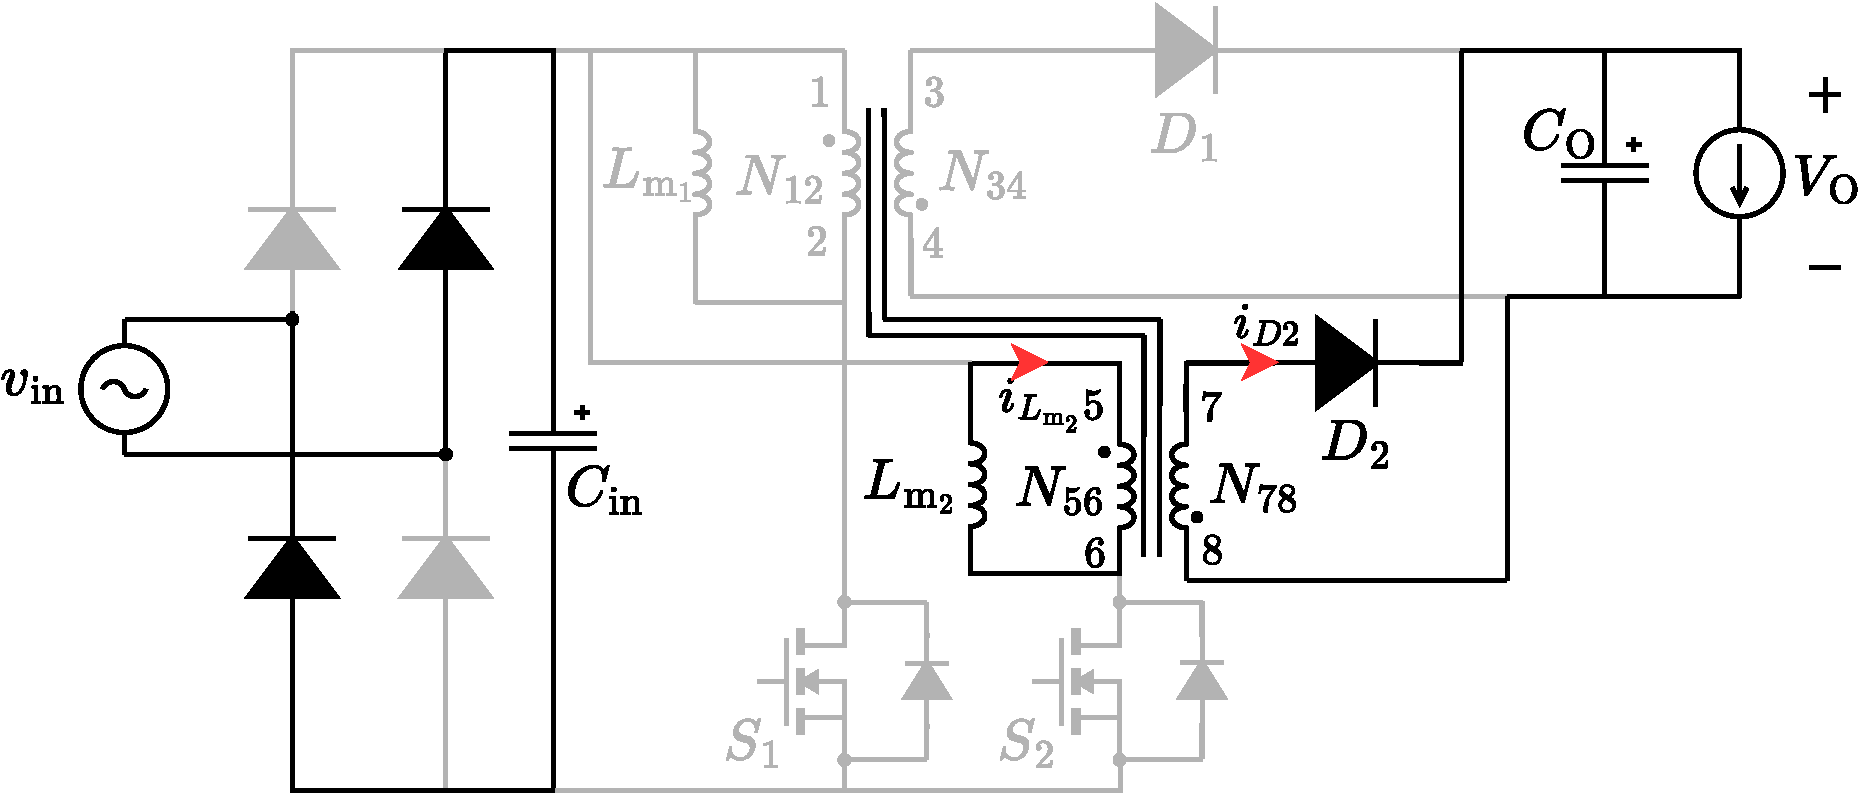
\includegraphics[width=\linewidth]{Figures_v2/Fig3f.pdf}%
        }
    \end{minipage}
    
    \caption{Operational principle of the two-phased interleaved flyback rectifier with the proposed integrated transformer at $D \le 0.5 \frac{n V_{\mathrm{o}}}{V_{\mathrm{in}_{\mathrm{max}}}}$. There are six distinct operational modes shown: (a) Mode 1 ($t_1 < t < t_2$), (b) Mode 2 ($t_2 < t < t_3$), (c) Mode 3 ($t_3 < t < t_4$), (d) Mode 4 ($t_4 < t < t_5$), (e) Mode 5 ($t_5 < t < t_6$), and (f) Mode 6 ($t_6 < t < t_7$).}
    \label{fig:operation_modes}
\end{figure*}

\begin{equation}
\label{eq:discharge}
t_{\mathrm{dis}} = \frac{V_{\mathrm{in}_{\mathrm{max}}} DT_{\mathrm{s}}}{n V_{\mathrm{o}}}
\end{equation}
with $T_{\mathrm{s}}$ as the switching period.

\begin{figure}[htbp]
\centering
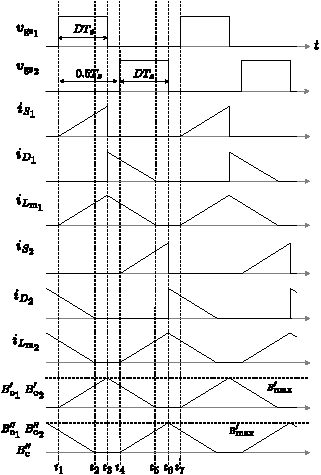
\includegraphics[width=\columnwidth]{Figures_v2/Fig4.pdf}

\caption{Key waveforms in the operation of the two-phase interleaved flyback rectifier with the proposed transformer, with $D \le 0.5 \frac{n V_{\mathrm{o}}}{V_{\mathrm{in}_{\mathrm{max}}}}$. }
\label{fig:4}
\end{figure}

To describe the magnetic state of the core, the superposition principle is used, as shown in Fig. \ref{fig:5a}. The magnetic flux density component $B'$ is generated by the positive cycle transformer defined as $N_{12}-N_{34}$. The magnetic flux density component $B''$ represents the component generated by the negative cycle transformer defined as $N_{56}-N_{78}$. The total flux in any leg is the algebraic sum of these components. This superposition determines the peak flux density required for the core design, which is analyzed in detail in Section II-B.

Modes 1, 2, and 3 in Fig. \ref{fig:mode_1}-\ref{fig:mode_3} cover the operation during the positive AC input into the rectifier, while Modes 4, 5, and 6 in Fig. \ref{fig:mode_4}--\ref{fig:mode_6} describe the operation during the negative AC input. For the following modes, $B'_{\mathrm{o}_1}$, $B'_{\mathrm{o}_2}$ and $B'_{\mathrm{c}}$ represent the magnetic flux densities in the respective left, right, and center legs of the core caused by the transformer active in positive AC input $N_{12}-N_{34}$, respectively, which are shown visually in Fig. \ref{fig:5b}. On the other hand, $B''_{\mathrm{o}_1}$, $B''_{\mathrm{o}_2}$ and $B''_{\mathrm{c}}$ represent the magnetic flux densities in the respective left, right, and center legs of the core caused by the transformer active in negative AC input $N_{56}-N_{78}$, respectively, which are detailed visually in Fig. \ref{fig:5c}.

\subsubsection*{\textup{1) Mode 1 ($t_1 < t < t_2$, \textup{Fig. \ref{fig:mode_1}})}}
At time $t_1$, switch $S_1$ turns on and $S_2$ remains off. The transformer $N_{12}-N_{34}$ begins storing energy in its magnetizing inductance. Its magnetizing current $i_{L_{\mathrm{m}_1}}$ and the corresponding flux densities in the outer legs $B'_{\mathrm{o}_1}$ and $B'_{\mathrm{o}_2}$ linearly increase from zero. Simultaneously, transformer $N_{56}-N_{78}$ completes its discharge phase, with its magnetizing current $i_{L_{\mathrm{m}_2}}$ and secondary diode current $i_{\mathrm{D}_2}$ decreasing to zero at $t_2$.

\subsubsection*{\textup{2) Mode 2 ($t_2 < t < t_3$, \textup{Fig. \ref{fig:mode_2}})}}
Mode 2 starts right after transformer $N_{56}-N_{78}$ completes its discharging phase, which means its associated currents $i_{\mathrm{D}_2}$, $i_{L_{\mathrm{m}_2}}$, and flux densities $B''_{\mathrm{o}_1}$, $B''_{\mathrm{o}_2}$ and $B''_{\mathrm{c}}$ are zero. Now, with $S_1$ still on, transformer $N_{12}-N_{34}$ continues storing energy until $i_{L_{\mathrm{m}_1}}$ reaches its peak value at $t_3$. The peak primary current in the positive cycle $i_{\mathrm{S}_{1_{\mathrm{pk}}}}$ is given by \eqref{eq:1}:
\begin{equation}
\label{eq:1}
i_{\mathrm{S}_{1_{\mathrm{pk}}}} = \frac{V_{\mathrm{in}} \cdot DT_{\mathrm{s}}}{L_{\mathrm{m}_1}}
\end{equation}
where $V_{\mathrm{in}}$ is the input voltage, $D$ is the duty cycle, $T_{\mathrm{s}}$ is the switching period, and $L_{\mathrm{m}_1}$ is the magnetizing inductance of transformer $N_{12}-N_{34}$. Consequently, the flux densities $B'_{\mathrm{o}_1}$ and $B'_{\mathrm{o}_2}$ also reach their peak values $B'_{o_{\mathrm{pk}}}$ which are given by \eqref{eq:2}:
\begin{equation}
\label{eq:2}
B'_{\mathrm{o}_{\mathrm{pk}}} = \frac{L_{\mathrm{m}_1} i_{\mathrm{S}_{1_{\mathrm{pk}}}}}{N_{12} A_{\mathrm{o}}}
\end{equation}
with $N_{12}$ as the number of turns in the primary side of the active transformer and $A_{\mathrm{o}}$ is the cross-sectional area of the outer-leg, where the transformer $N_{12}-N_{34}$ is wound.

\subsubsection*{\textup{3) Mode 3 ($t_3 < t < t_4$, \textup{Fig. \ref{fig:mode_3}})}}
Mode 3 starts right after transformer $N_{12}-N_{34}$ finishes charging. At $t_3$, Switch $S_1$ turns off, initiating the discharge phase of transformer $N_{12}-N_{34}$. The magnetizing current $i_{L_{\mathrm{m}_1}}$, diode current $i_{\mathrm{D}_1}$, and flux densities $B'_{\mathrm{o}_1}$ and $B'_{\mathrm{o}_2}$ begin to decrease linearly. Transformer $N_{56}-N_{78}$ remains inactive in this period. 

In Modes 1-3, the magnetomotive force and magnetic resistance of both outer legs are equal. The magnetic flux in the center leg is canceled. This causes no electromotive force generated in transformer $N_{56}-N_{78}$. Therefore, the transformer formed by the outer legs operates independently from the transformer in the center leg. The integrated transformer is equivalent to that of Fig. \ref{fig:5b} and its equivalent magnetic circuit is shown in Fig. \ref{fig:6a}.

\subsubsection*{\textup{4) Mode 4 ($t_4 < t < t_5$, \textup{Fig. \ref{fig:mode_4}})}}
Mode 4 operates similarly to the positive cycle. Switch $S_2$ turns on at $t_4$ and $S_1$ remains off. Transformer $N_{56}-N_{78}$ stores energy in its magnetizing inductance. Its current $i_{L_{\mathrm{m}_2}}$ and the corresponding flux densities $B''_{\mathrm{o}_1}$, $B''_{\mathrm{c}}$ and $B''_{\mathrm{o}_2}$ linearly increase. Simultaneously, transformer $N_{12}-N_{34}$ completes its discharge phase, with $i_{L_{\mathrm{m}_1}}$ and $i_{\mathrm{D}_1}$ decreasing to zero at $t_5$.

\subsubsection*{\textup{5) Mode 5 ($t_5 < t < t_6$, \textup{Fig. \ref{fig:mode_5}})}}
Mode 5 starts after the discharge of transformer $N_{12}-N_{34}$ completes. Now, with Switch $S_2$ still on, transformer $N_{56}-N_{78}$ continues storing energy until $i_{L_{\mathrm{m}_2}}$ reaches its peak value at $t_6$. The peak primary current in the negative cycle $i_{\mathrm{S}_{2_{\mathrm{pk}}}}$ is given by \eqref{eq:3}:
\begin{equation}
\label{eq:3}
i_{\mathrm{S}_{2_{\mathrm{pk}}}} = \frac{V_{\mathrm{in}} \cdot DT_{\mathrm{s}}}{L_{\mathrm{m}_2}}
\end{equation}
where $L_{\mathrm{m}_2}$ is the magnetizing inductance of transformer $N_{56}-N_{78}$. Consequently, the flux densities $B''_{\mathrm{o}_1}$, $B''_{\mathrm{c}}$, and $B''_{\mathrm{o}_2}$ also reach their peak values. The peak value of $B''_{\mathrm{c}_{\mathrm{pk}}}$ is given by \eqref{eq:4}:
\begin{equation}
\label{eq:4}
B''_{\mathrm{c}_{\mathrm{pk}}} = B''_{\mathrm{o}_{\mathrm{pk}}} = \frac{L_{\mathrm{m}_2} i_{\mathrm{S}_{2_{\mathrm{pk}}}}}{N_{56} A_{\mathrm{c}}}
\end{equation}
with $N_{56}$ as the number of turns in the primary side of the active transformer and $A_{\mathrm{c}}$ is the cross-sectional area of the center leg where the transformer $N_{56}-N_{78}$ is wound.

\subsubsection*{\textup{6) Mode 6 ($t_6 < t < t_7$, \textup{Fig. \ref{fig:mode_6}})}}
Switch $S_2$ turns off, initiating the discharge phase of transformer $N_{56}-N_{78}$. The currents $i_{L_{\mathrm{m}_2}}, i_{\mathrm{D}_2},$ and flux densities $B''_{\mathrm{o}_1}$, $B''_{\mathrm{c}}$ and $B''_{\mathrm{o}_2}$ begin to decrease linearly. Transformer $N_{12}-N_{34}$ remains inactive.

For modes 4-6, since the magnetic resistance of both outer legs is equal, the magnetic flux is divided equally into both outer legs. Furthermore, since the number of turns of both outer legs is equal and wound in an opposite polarity, the electromotive force generated in $N_{12}-N_{34}$ is canceled. Therefore, the transformer formed by the center leg operates independently from the transformer in the outer leg, and the integrated transformer is equivalent to that of Fig. \ref{fig:5c}. The equivalent magnetic circuit for this case is shown in Fig. \ref{fig:6b}.

The proposed winding structure achieves zero magnetic coupling between the two transformers. Consequently, the distinct magnetic circuits share a single core without magnetic interference. Each transformer maintains independent operation despite the physical integration. This structure eliminates the need for two discrete magnetic components. As a result, the total volume of the magnetic components is significantly reduced.

\begin{figure}[htbp]
\centering
% (a) Top circuit
        \subfloat[]{
        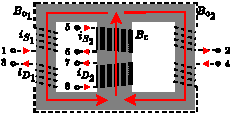
\includegraphics[width=0.6\columnwidth]{Figures_v2/Fig5a.pdf} % Make sure this file exists
        \label{fig:5a}
        }
        \\ % This double backslash forces the next image to the line below (vertical stack)
        % (b) Middle circuit
        \subfloat[]{
        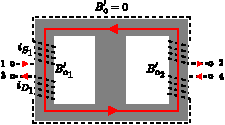
\includegraphics[width=0.6\columnwidth]{Figures_v2/Fig5b.pdf}
        \label{fig:5b}
        }
        \\
        \subfloat[]{
        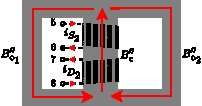
\includegraphics[width=0.53\columnwidth]{Figures_v2/Fig5c.pdf}
        \label{fig:5c}
        }
        \caption{The proposed integrated transformer during the two phases of the converter, with the flux density components in each leg illustrated in (a). (b) is realized during the positive AC cycle, while (c) is realized during the negative cycle.}
\end{figure}
\begin{figure}[htbp]
\centering
% (a) Top circuit
        \subfloat[]{
        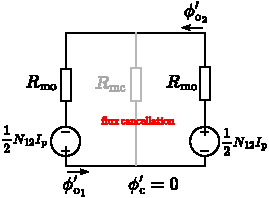
\includegraphics[width=0.6\columnwidth]{Figures_v2/Fig6a.pdf} % Make sure this file exists
        \label{fig:6a}
        }
        \\ % This double backslash forces the next image to the line below (vertical stack)
        % (b) Middle circuit
        \subfloat[]{
        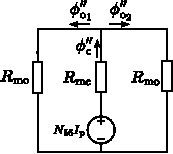
\includegraphics[width=0.43\columnwidth]{Figures_v2/Fig6b.pdf}\hspace{0.7cm}
        \label{fig:6b}
        }
        
        \caption{Equivalent magnetic circuits for the proposed transformer. (a) shows the equivalent magnetic circuit for $N_{12}-N_{34}$, while (b) shows the equivalent magnetic circuit for $N_{56}-N_{78}$.}
\end{figure}

\subsection{Saturation Magnetic Flux Density Analysis}
\begin{figure*}[htbp]
    \centering
    % The figure spans two columns, so we use figure*
    
    % --- (a) Case 1 ---
    % \subfloat[] automatically generates the "(a)" label. 
    % We leave the bracket empty [] because the text "Case 1" is in the main caption, not the sub-label.
    \subfloat[\label{fig:case1}]{%
        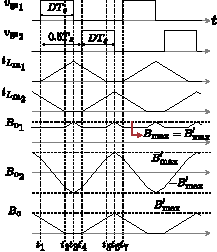
\includegraphics[width=0.32\textwidth]{Figures_v2/Fig7a.pdf}%
    }
    \hfill % Adds flexible space between images
    % --- (b) Case 2 ---
    \subfloat[\label{fig:case2}]{%
        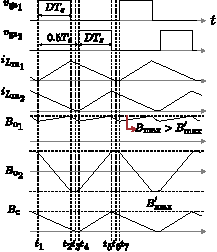
\includegraphics[width=0.32\textwidth]{Figures_v2/Fig7b.pdf}%
    }
    \hfill
    % --- (c) Case 3 ---
    \subfloat[\label{fig:case3}]{%
        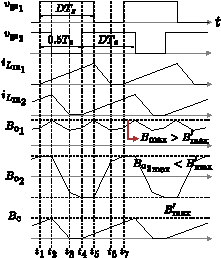
\includegraphics[width=0.32\textwidth]{Figures_v2/Fig7c.pdf}%
    }
    
    \caption{Theoretical, superimposed magnetic flux density waveforms in the integrated transformer during circuit operations: (a) Case 1, (b) Case 2, and (c) Case 3.}
    \label{fig:flux_waveforms}
\end{figure*}

The circuit operation is classified into three patterns determined by the duty cycle $D$ and the boundary condition $D \le 0.5 \frac{n V_{\mathrm{o}}}{V_{\mathrm{in}_{\mathrm{max}}}}$. This classification, illustrated in Fig. 7, arises because the integrated single-core structure permits simultaneous magnetizing current flow in multiple active windings, resulting in distinct flux superposition compared to conventional discrete transformers. The manner of superposition due to the magnetizing current can be controlled by $t_{\mathrm{dis}}$. Consequently, the saturation magnetic flux density $B_{\mathrm{sat}}$ is a critical parameter for the transformer geometry. The flux density in each leg is examined further using the principle of superposition, with the expressions of the superimposed flux densities in the left, right and center legs shown in \eqref{eq:5}-\eqref{eq:7}, represented as $B_{\mathrm{o}_1}$, $B_{\mathrm{o}_2}$ and $B_{\mathrm{c}}$ respectively:
\begin{align}
B_{\mathrm{o}_1} &= B'_{\mathrm{o}_1} + B''_{\mathrm{o}_1} \label{eq:5}\\
B_{\mathrm{o}_2} &= B'_{\mathrm{o}_2} - B''_{\mathrm{o}_2} \label{eq:6}\\
B_{\mathrm{c}} &= B''_{\mathrm{c}} \label{eq:7}
\end{align}

\subsubsection*{\textup{Case 1: $D < 0.5$ and $D \le 0.5 \frac{n V_{\mathrm{o}}}{V_{\mathrm{in}_{\mathrm{max}}}}$}}
The waveforms in Fig. 4 represent the circuit operation for Case 1. As shown, flux cancellation does not occur in the outer legs; however, the magnitude of the peak flux density remains uniform across all legs. If the magnetizing current of one phase reaches zero before the magnetizing current of the other phase reaches its peak, then the saturation magnetic flux density of the core across all the phases, $B_{\mathrm{max}}$, is equal to $B'_{\mathrm{max}}$. This condition is satisfied when $D$ is expressed by \eqref{eq:8}.
\begin{equation}
\label{eq:8}
D \le 0.5 \frac{n V_{\mathrm{o}}}{V_{\mathrm{in}_{\mathrm{max}}}}
\end{equation}

\subsubsection*{\textup{Case 2: $D < 0.5$ and $D > 0.5 \frac{n V_{\mathrm{o}}}{V_{\mathrm{in}_{\mathrm{max}}}}$}}
In this scenario, the magnetizing current of one phase does not reach zero before the subsequent phase reaches its peak. The saturation flux density across all phases can be derived as follows: At $t_2$, $B'_{\mathrm{o}_1} = B'_{\mathrm{max}}$. Moreover, $B''_{\mathrm{o}_1}(t_2) = B'_{\mathrm{o}_1}(t_5)$ and is expressed in \eqref{eq:9}:
\begin{equation}
\label{eq:9}
B''_{\mathrm{o}_1}(t_2) = B'_{\mathrm{o}_1}(t_5) = B'_{\mathrm{max}} - \frac{B'_{\mathrm{max}}}{t_6 - t_2}(t_5 - t_2)
\end{equation}
With $t_5 = 0.5 T_{\mathrm{s}} + t_2$ and $t_2 = D T_{\mathrm{s}}$. The peak $i_{L_{\mathrm{m}_{1_{\mathrm{pk}}}}}$ can be rewritten as in \eqref{eq:10}:
\begin{equation}
\label{eq:10}
i_{L_{{{\mathrm{m}_1}_{\mathrm{pk}}}}} = \frac{V_{\mathrm{in}_{\mathrm{max}}}}{L_{\mathrm{m}}} D T_{\mathrm{s}} = \frac{n V_{\mathrm{o}}}{L_{\mathrm{m}}}(t_6 - t_2)
\end{equation}
In this case, \eqref{eq:8} is not satisfied, and this results in $B_{\mathrm{max}}$ in the left outer leg exceeding $B'_{\mathrm{max}}$ in the center leg, as expressed in \eqref{eq:11}:
\begin{equation}
\label{eq:11}
B_{\mathrm{max}} = \left(2 - \frac{0.5 n V_{\mathrm{o}}}{V_{\mathrm{in}_{\mathrm{max}}} D}\right) B'_{\mathrm{max}}
\end{equation}

\subsubsection*{\textup{Case 3: $D > 0.5$}}
In this case, $B_{\mathrm{max}}$ in the left outer leg consistently exceeds $B'_{\mathrm{max}}$. By analysis similar to Case 2, $B_{\mathrm{max}}$ is derived as \eqref{eq:12}:
\begin{equation}
\label{eq:12}
B_{\mathrm{max}} = \left(1 + \frac{D - 0.5}{D}\right) B'_{\mathrm{max}}
\end{equation}

Because the flyback is interleaved, it is expected that the rectifier will primarily operate at $D < 0.5$ (Case 1 or 2).

\subsection{Design Method of the Proposed Integrated Transformer}
\begin{figure}[htbp]
\centering
% (a) Top circuit
        \subfloat[]{
        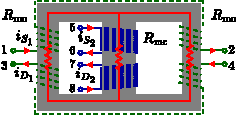
\includegraphics[width=0.6\columnwidth]{Figures_v2/Fig8a.pdf} % Make sure this file exists
        \label{fig:8a}
        }
        \\ % This double backslash forces the next image to the line below (vertical stack)
        % (b) Middle circuit
        \subfloat[]{
        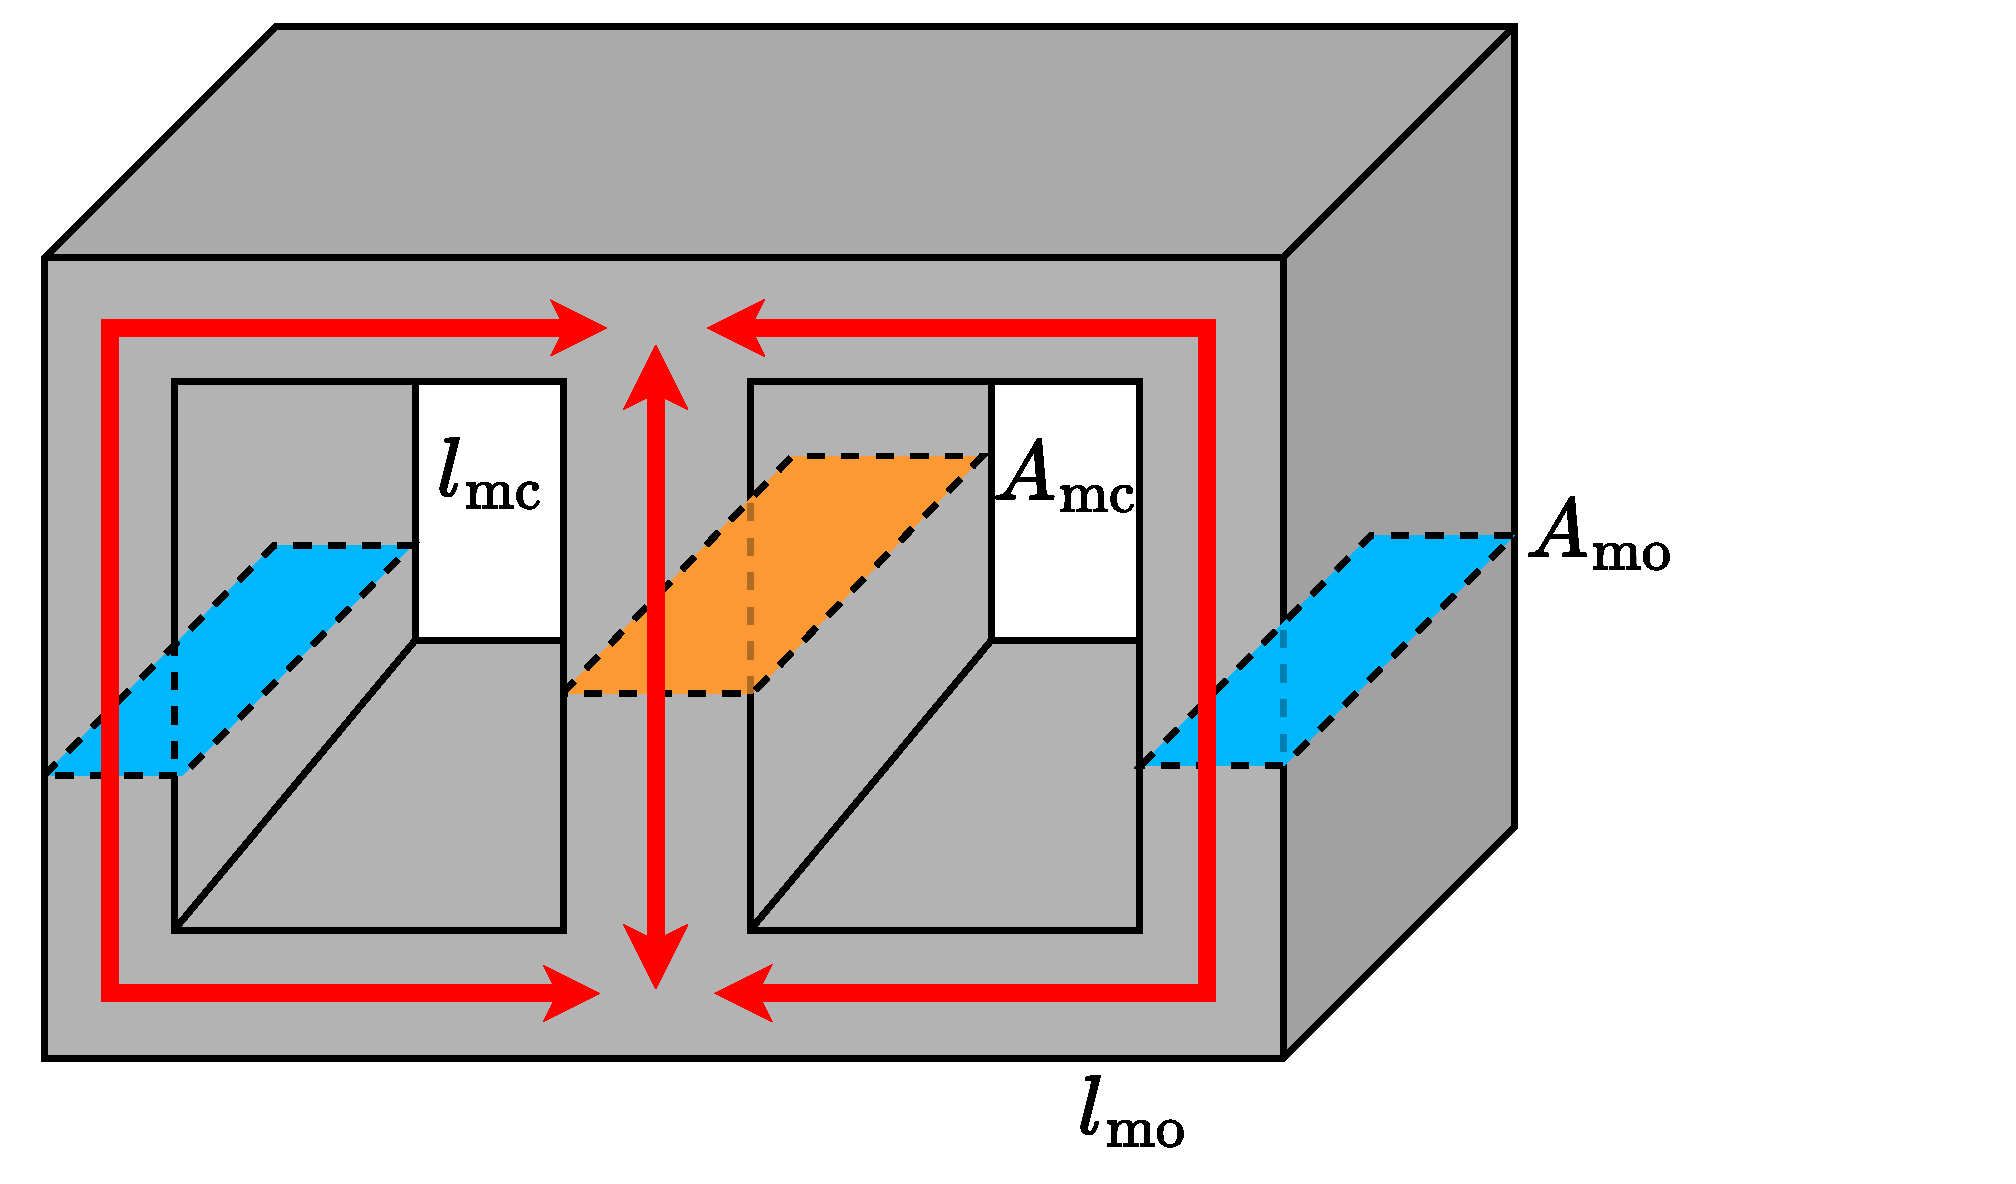
\includegraphics[width=0.58\columnwidth]{Figures_v2/Fig8b.pdf}
        \label{fig:8b}
        }
        
        \caption{EE core configuration: (a) magnetic resistances of the transformer ($R_{\mathrm{mo}}$ for the outer legs, $R_{\mathrm{mc}}$ for the center leg), and (b) effective cross-sectional area ($A_{\mathrm{mo}}$ for the outer legs, $A_{\mathrm{mc}}$ for the center leg) and effective magnetic path length $l_{\mathrm{mo}}$ for the outer legs, $l_{\mathrm{mc}}$ for the center leg.}
\end{figure}
\begin{figure}[htbp]
\centering
% (a) Top circuit
        \subfloat[]{
        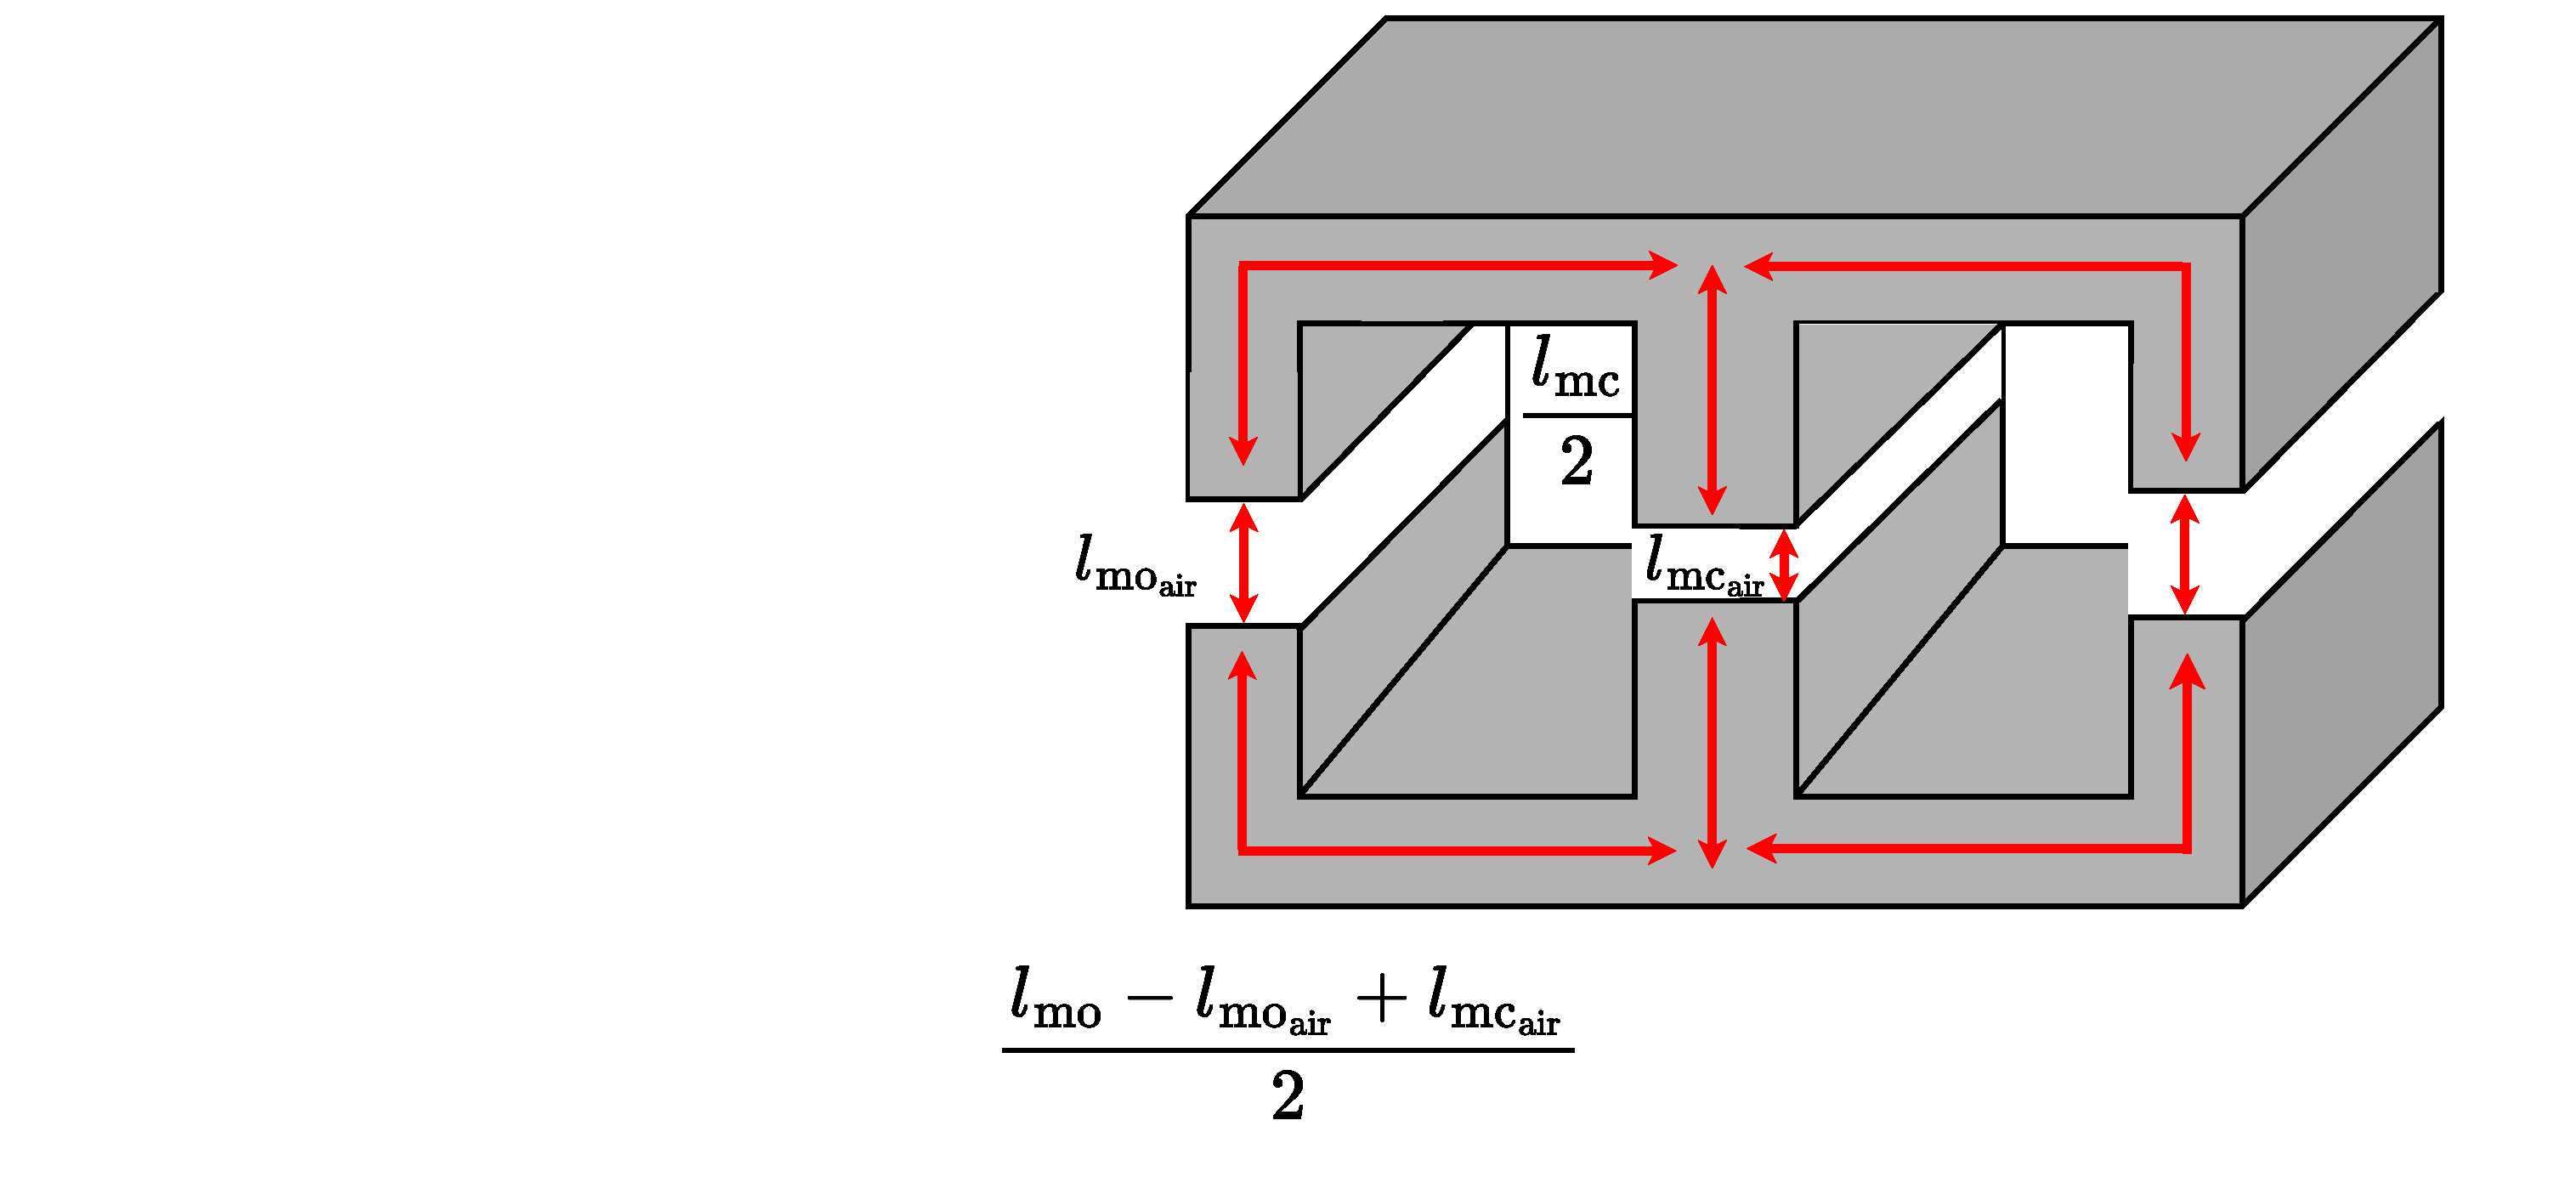
\includegraphics[width=0.75\columnwidth]{Figures_v2/Fig9a.pdf} % Make sure this file exists
        \label{fig:9a}
        }
        \\ % This double backslash forces the next image to the line below (vertical stack)
        % (b) Middle circuit
        \subfloat[]{
        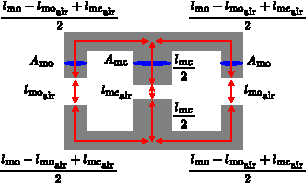
\includegraphics[width=0.8\columnwidth]{Figures_v2/Fig9b.pdf}
        \label{fig:9b}
        }
        
        \caption{EE core configuration with air gaps: (a) setup when $l_{\mathrm{mo}_{\mathrm{air}}} < l_{\mathrm{mc}_{\mathrm{air}}}$ and (b) setup when $l_{\mathrm{mo}_{\mathrm{air}}} > l_{\mathrm{mc}_{\mathrm{air}}}$.}
\end{figure}

A turns ratio $n$ is selected in consideration of the maximum rated voltages of the switches used. A duty cycle $D$ is selected to decide an operating pattern. $B'_{\mathrm{max}}$ is calculated from the chosen core material. Afterwards, the magnetizing inductance, $L_{\mathrm{m}_1}=L_{\mathrm{m}_2}=L_{\mathrm{m}}$ in this paper, is calculated from the circuit specifications. A core is chosen using the area-product method. The number of turns is calculated using $B'_{\mathrm{max}}$ and the peak primary side current $I_{\mathrm{pri}_{\mathrm{pk}}}$ as shown in \eqref{eq:13} and \eqref{eq:14}:
\begin{equation}
\label{eq:13}
N_{34} \ge \frac{L_{\mathrm{m}} I_{\mathrm{pri}_{\mathrm{pk}}}}{n A_{\mathrm{mo}} B'_{\mathrm{max}}}, \quad N_{12} = n N_{34}
\end{equation}
\begin{equation}
\label{eq:14}
N_{78} \ge \frac{L_{\mathrm{m}} I_{\mathrm{pri}_{\mathrm{pk}}}}{n A_{\mathrm{mc}} B'_{\mathrm{max}}}, \quad N_{56} = n N_{78}
\end{equation}

The magnetic resistances of the outer legs $R_{\mathrm{mo}}$ and the central leg $R_{\mathrm{mc}}$ are obtained from a magnetic circuit analysis of the integrated transformer in its separated components. The transformer $N_{12}-N_{34}$ is only made of the outer legs as shown in Fig. \ref{fig:8b} while that of $N_{56}-N_{78}$ is made of all the legs. The magnetizing inductances implied by $N_{12}-N_{34}$ and $N_{56}-N_{78}$ are shown in \eqref{eq:15} and \eqref{eq:16} respectively.
\begin{align}
L_{\mathrm{m}} &= \frac{N_{12}^2}{2 R_{\mathrm{mo}}} \label{eq:15}\\
L_{\mathrm{m}} &= \frac{N_{56}^2}{R_{\mathrm{mc}} + 0.5 R_{\mathrm{mo}}} \label{eq:16}
\end{align}
$R_{\mathrm{mo}}$ and $R_{\mathrm{mc}}$ are obtained from \eqref{eq:17} and \eqref{eq:18}:
\begin{align}
R_{\mathrm{mo}} &= \frac{N_{12}^2}{2 L_{\mathrm{m}}} \label{eq:17}\\
R_{\mathrm{mc}} &= \frac{(2 N_{56} - N_{12})(2 N_{56} + N_{12})}{4 L_{\mathrm{m}}} \label{eq:18}
\end{align}

Finally, an air gap was also inserted in each of the legs to provide the desired resistance. Non-equal length air gaps were placed in the transformer. There are two cases, one in which the air gaps in the outer legs $l_{\mathrm{mo}_{\mathrm{air}}}$ are longer than the air gap in the center leg $l_{\mathrm{mc}_{\mathrm{air}}}$, and one in which $l_{\mathrm{mc}_{\mathrm{air}}}$ is longer than $l_{\mathrm{mo}_{\mathrm{air}}}$.

\subsubsection*{\textup{Case 1: $l_{\mathrm{mo}_{\mathrm{air}}} > l_{\mathrm{mc}_{\mathrm{air}}}$}}
Given the setup in Fig. \ref{fig:9a}, the corresponding magnetic resistances of the outer and center legs are shown in \eqref{eq:19} and \eqref{eq:20} and can be solved for the corresponding air gap lengths as shown in \eqref{eq:21} and \eqref{eq:22}.
\begin{align}
R_{\mathrm{mo}} &= \frac{l_{\mathrm{mo}} - l_{\mathrm{mo}_{\mathrm{air}}} + l_{\mathrm{mc}_{\mathrm{air}}}}{\mu_r \mu_0 A_{\mathrm{mo}}} + \frac{l_{\mathrm{mo}_{\mathrm{air}}}}{\mu_0 A_{\mathrm{mo}}} \label{eq:19}\\
R_{\mathrm{mc}} &= \frac{l_{\mathrm{mc}}}{\mu_r \mu_0 A_{\mathrm{mc}}} + \frac{l_{\mathrm{mc}_{\mathrm{air}}}}{\mu_0 A_{\mathrm{mc}}} \label{eq:20}\\
l_{\mathrm{mo}_{\mathrm{air}}} &= \frac{\mu_0 (\mu_r A_{\mathrm{mo}} R_{\mathrm{mo}} - A_{\mathrm{mc}} R_{\mathrm{mc}}) + \frac{l_{\mathrm{mc}}}{\mu_r} - l_{\mathrm{mo}}}{\mu_r - 1} \label{eq:21}\\
l_{\mathrm{mc}_{\mathrm{air}}} &= \mu_0 A_{\mathrm{mc}} R_{\mathrm{mc}} - \frac{l_{\mathrm{mc}}}{\mu_r} \label{eq:22}
\end{align}

\subsubsection*{\textup{Case 2: $l_{\mathrm{mc}_{\mathrm{air}}} > l_{\mathrm{mo}_{\mathrm{air}}}$}}
Given the setup in Fig. \ref{fig:9b}, the corresponding magnetic resistances are shown in \eqref{eq:23} and \eqref{eq:24} and air gap lengths in \eqref{eq:25} and \eqref{eq:26}.
\begin{align}
R_{\mathrm{mo}} &= \frac{l_{\mathrm{mo}}}{\mu_r \mu_0 A_{\mathrm{mo}}} + \frac{l_{\mathrm{mo}_{\mathrm{air}}}}{\mu_0 A_{\mathrm{mo}}} \label{eq:23}\\
R_{\mathrm{mc}} &= \frac{l_{\mathrm{mc}} - l_{\mathrm{mc}_{\mathrm{air}}} + l_{\mathrm{mo}_{\mathrm{air}}}}{\mu_r \mu_0 A_{\mathrm{mc}}} + \frac{l_{\mathrm{mc}_{\mathrm{air}}}}{\mu_0 A_{\mathrm{mc}}} \label{eq:24}\\
l_{\mathrm{mo}_{\mathrm{air}}} &= \mu_0 A_{\mathrm{mo}} R_{\mathrm{mo}} - \frac{l_{\mathrm{mo}}}{\mu_r} \label{eq:25}\\
l_{\mathrm{mc}_{\mathrm{air}}} &= \frac{\mu_0 (\mu_r A_{\mathrm{mc}} R_{\mathrm{mc}} - A_{\mathrm{mo}} R_{\mathrm{mo}}) + \frac{l_{\mathrm{mo}}}{\mu_r} - l_{\mathrm{mc}}}{\mu_r - 1} \label{eq:26}
\end{align}


\section{Simulation Verification of Proposed Design}

\subsection{Simulation Verification of the Proposed Design Method}
To ensure the validity and operation of the proposed integrated transformer, a simulation of the two-phase interleaved flyback rectifier was first performed in PLECS Standalone 4.9.4, with the diagram shown in Fig. \ref{fig:10a}. Clamped RCD Snubber circuits ($C_{\mathrm{sn}_1}, D_{\mathrm{sn}_1}, R_{\mathrm{sn}_1}$ and $C_{\mathrm{sn}_2}, D_{\mathrm{sn}_2}, R_{\mathrm{sn}_2}$) were also added to the circuit for protection against surge voltage \cite{ref15, ref16} caused by the leakage inductance and the switch capacitance at the turn-off time of $S_1$ and $S_2$. An integrated transformer, shown in Fig. 10(b), was also designed using the proposed method. The circuit and transformer were designed with the condition given by \eqref{eq:8}, and will thus be verified in this study. The specifications of the two-phase interleaved flyback rectifier and transformer for the simulation verification are shown in Tables \ref{tab:sim_rectifier} and \ref{tab:sim_transformer} respectively. The duty cycle is calculated using \eqref{eq:27} \cite{ref8}.
\begin{equation}
\label{eq:27}
D = \frac{2}{V_{\mathrm{in}_{\mathrm{pk}}}} \sqrt{\frac{0.5 L_{\mathrm{m}} P_{\mathrm{o}}}{T_{\mathrm{s}}}}
\end{equation}

\begin{table}[htbp]
    \caption{Simulation Specifications of the Prototype Two-Phase Interleaved Flyback Rectifier}
    \centering
    \footnotesize
    \setlength{\tabcolsep}{3pt} % Slightly tighter spacing to handle long text
    \begin{tabular}{ccc}
        \hline
        \textbf{Item} & \textbf{Symbol} & \textbf{Value} \\
        \hline \hline
        AC input voltage & $v_{\mathrm{in}}$ & 100 V \\
        Maximum rated power & $P_{\mathrm{out}}$ & 240 W \\
        Output voltage & $V_{\mathrm{out}}$ & 48 V \\
        Switching frequency & $f_{\mathrm{s}}$ & 100 kHz \\
        Input capacitor & $C_{\mathrm{in}}$ & 1 $\mu$F \\
        Output capacitor & $C_{\mathrm{out}}$ & 2 x 1mF (parallel) \\
        Snubber capacitor & $C_{\mathrm{sn}_1}, C_{\mathrm{sn}_2}$ & 2.2 nF \\
        Snubber resistor & $R_{\mathrm{sn}_1}, R_{\mathrm{sn}_2}$ & 30 k$\Omega$ \\
        \hline
    \end{tabular}
    \label{tab:sim_rectifier}
\end{table}

\begin{table}[htbp]
    \caption{Prototype Integrated Transformer Specifications}
    \centering
    \footnotesize
    \setlength{\tabcolsep}{4pt} 
    \begin{tabular}{ccc}
        \hline
        \textbf{Item} & \textbf{Symbol} & \textbf{Value} \\
        \hline \hline
        Magnetic core & - & OP44721EC \\
        Relative permeability & $mu_r$ & 2500\\
        Magnetic path length (center leg) & $l_{\mathrm{mc}}$ & 31.7 mm\\
        Magnetic path length (outer leg) & $l_{\mathrm{mo}}$ & 71.4 mm\\
        Cross-sectional area (center leg) & $A_{\mathrm{mc}}$ & 243.4 mm$^2$ \\
        Cross-sectional area (outer leg) & $A_{\mathrm{mo}}$ & 117.6 $^2$\\
        Magnetizing inductance & $L_{\mathrm{m}_1}, L_{\mathrm{m}_2}$ & 82.8 $\mu$H \\
        Turn ratio & $n$ & 3 \\
        \multirow{2}{*}{Number of turns} & $N_{12}:N_{34}$ & 24:8 \\
                                         & $N_{56}:N_{78}$ & 18:6 \\
        Center leg air gap & $l_{\mathrm{gc}}$ & 0.650 mm \\
        Outer leg air gap & $l_{\mathrm{go}}$ & 0.500 mm \\
        Coupling coefficient of $N_{12}, N_{34}$ & $k_{N_{12},N_{34}}$ & 0.990 \\
        Coupling coefficient of $N_{56}, N_{78}$ & $k_{N_{56},N_{78}}$ & 0.990 \\
        Coupling coefficient of $N_{12}, N_{56}$ & $k_{N_{12},N_{56}}$ & 0.000 \\
        \hline
    \end{tabular}
    \label{tab:sim_transformer}
\end{table}

\begin{figure}[htbp]
\centering
% (a) Top circuit
        \subfloat[]{
        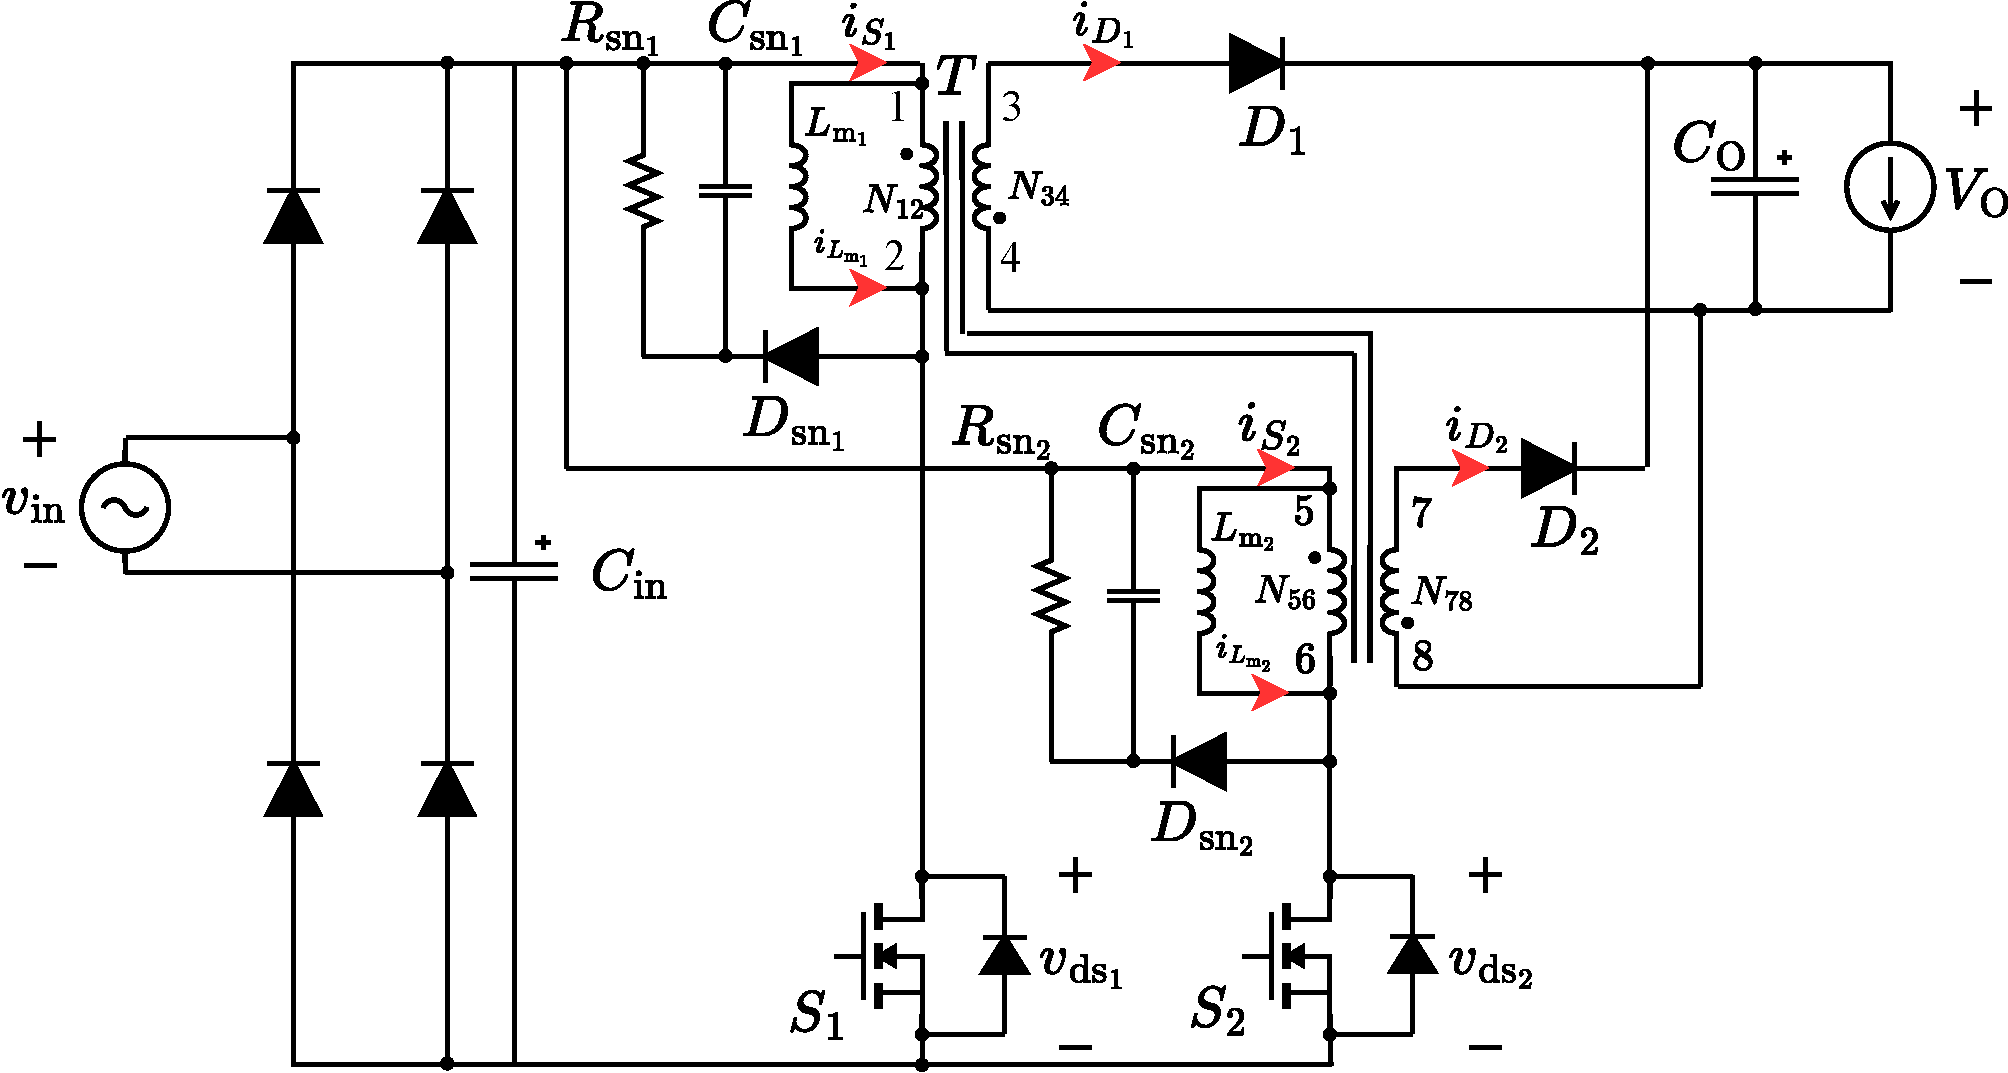
\includegraphics[width=\columnwidth]{Figures_v2/Fig10a.pdf} % Make sure this file exists
        \label{fig:10a}
        }
        \\ % This double backslash forces the next image to the line below (vertical stack)
        % (b) Middle circuit
        \subfloat[]{
        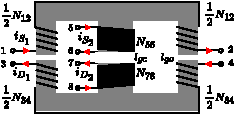
\includegraphics[width=0.6\columnwidth]{Figures_v2/Fig10b.pdf}
        \label{fig:10b}
        }
        
        \caption{Prototype two-phase interleaved flyback rectifier (a) with the proposed integrated transformer (b).}
\end{figure}

\subsection{Simulation Results}
Figure 11 shows waveforms from the simulation testing of the two-phase interleaved flyback rectifier with the proposed transformer at 240 W. Key waveforms of the circuit were observed from the simulation, which include $v_{\mathrm{gs}_1}$ and $v_{\mathrm{gs}_2}$, $i_{L_{\mathrm{m}_1}}$ and $i_{L_{\mathrm{m}_2}}$, and the fluxes $B_{\mathrm{o}_1}$, $B_{\mathrm{o}_2}$, and $B_{\mathrm{c}}$. Similar waveforms to that of Fig. \ref{fig:4} have been observed. Flux cancellation is observed in the center leg during the time that it is inactive, which then confirms the validity of the theoretical operation proposed in Section II. Moreover, the increase and decrease of fluxes were all linear, therefore confirming that there is indeed no magnetic coupling interference.

\begin{figure}[htbp]
\centering
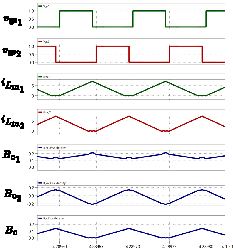
\includegraphics[width=0.8\columnwidth]{Figures_v2/Fig11.pdf} % Make sure this file exists
\caption{Key waveforms of the proposed two-phase interleaved flyback rectifier with the proposed integrated transformer in simulation.}
\label{fig:11}
\end{figure}

\section{Size Reduction Effect of the Proposed Transformer}
This section examines the size reduction effect by the integrated transformer. For this study, the conventional transformer is assumed to be the two separate transformers that facilitate isolation between the primary and secondary side. A representation is shown in Fig. \ref{fig:12a}, and its windings are represented in Fig. \ref{fig:13a}. The proposed integrated transformer is represented as shown in Fig. \ref{fig:12b} and its windings are shown in Fig. \ref{fig:13b}. The volume is compared by using the area-product (AP) method. The AP method utilizes the product between the core cross-sectional area, $A_{\mathrm{c}}$, and the window-area, $A_{\mathrm{w}}$, and is a fundamental core size for the application \cite{ref21}.
\begin{figure}[htbp]
\centering
% (a) Top circuit
        \subfloat[]{
        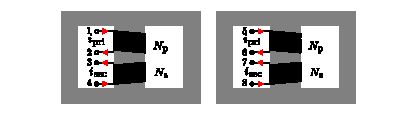
\includegraphics[width=0.9\columnwidth]{Figures_v2/Fig12a.pdf} % Make sure this file exists
        \label{fig:12a}}
        \\ % This double backslash forces the next image to the line below (vertical stack)
        % (b) Middle circuit
        \subfloat[]{
        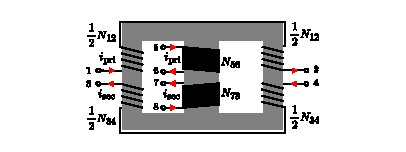
\includegraphics[width=0.6\columnwidth]{Figures_v2/Fig12b.pdf}
        \label{fig:12b}}
        
        \caption{Conventional (a) and proposed integrated transformer (b) used in the volume analysis.}
        \label{fig:12}
\end{figure}
\begin{figure}[htbp]
\centering
% (a) Top circuit
        \subfloat[]{
        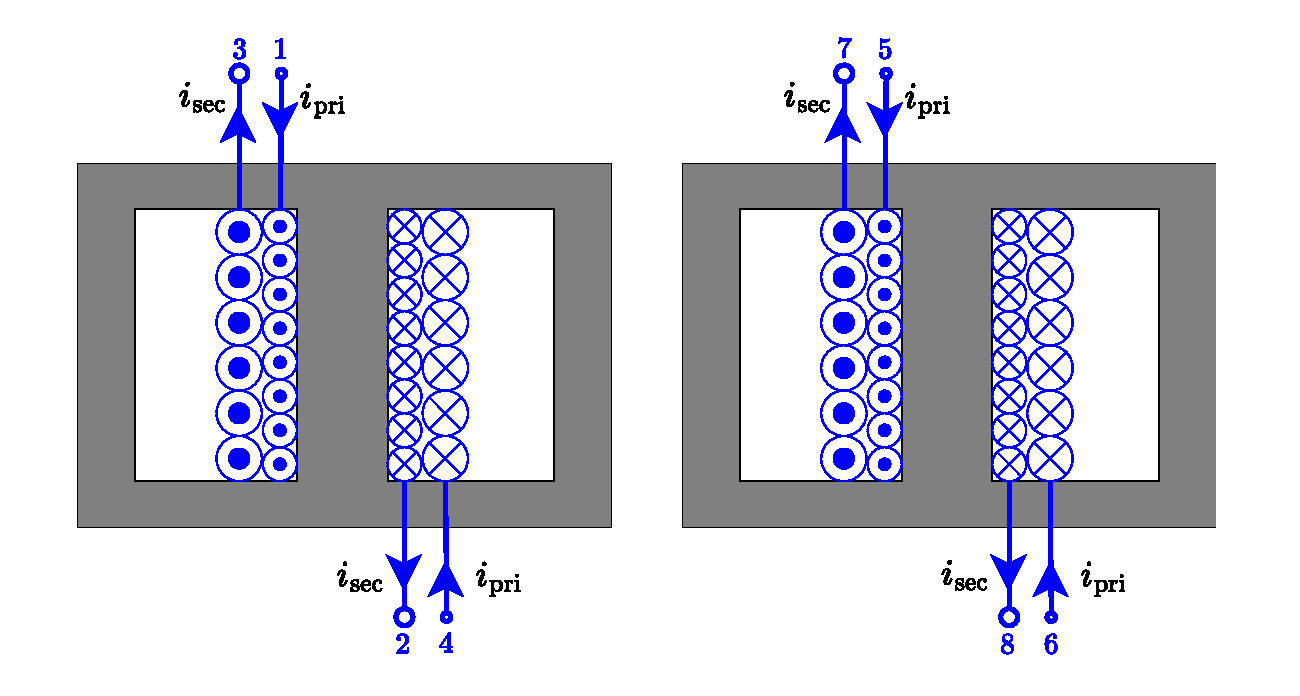
\includegraphics[width=0.9\columnwidth]{Figures_v2/Fig13a.pdf} % Make sure this file exists
        \label{fig:13a}
        }
        \\ % This double backslash forces the next image to the line below (vertical stack)
        % (b) Middle circuit
        \subfloat[]{
        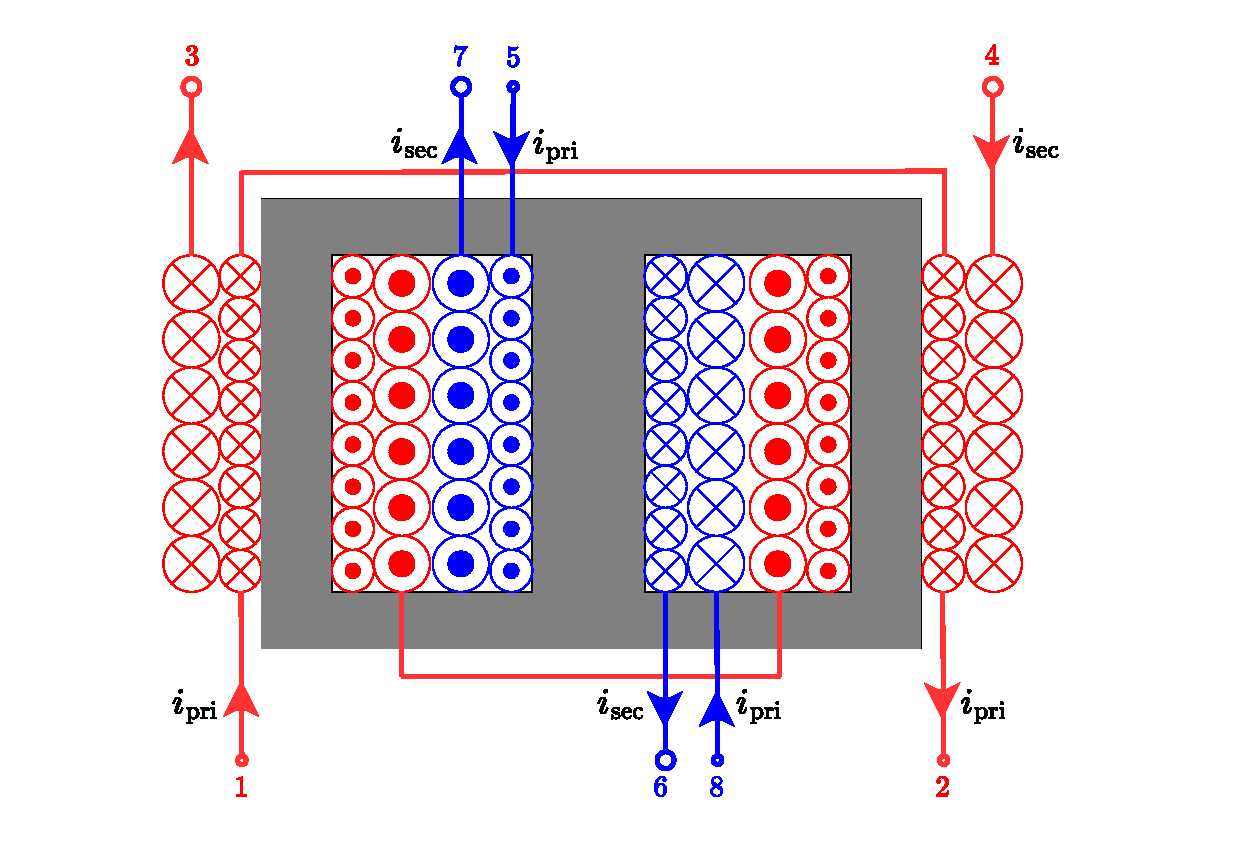
\includegraphics[width=0.6\columnwidth]{Figures_v2/Fig13b.pdf}
        \label{fig:13b}
        }
        
        \caption{Conventional (a) and proposed integrated transformer (b) used in the volume analysis, with the windings represented as well.}
        \label{fig:13}
\end{figure}

The EE-core was redesigned in such a way such that $A_{\mathrm{w}}$ and $A_{\mathrm{c}}$ are squares to allow for simpler analysis, as shown in Fig. \ref{fig:14} \cite{ref22}. Here, $A_{\mathrm{c}}$ is twice the area of the outer leg. This leads to $N_{12}$ and $N_{34}$ having twice as many turns as $N_{56}$ and $N_{78}$ respectively.

\begin{figure}[htbp]
\centering
        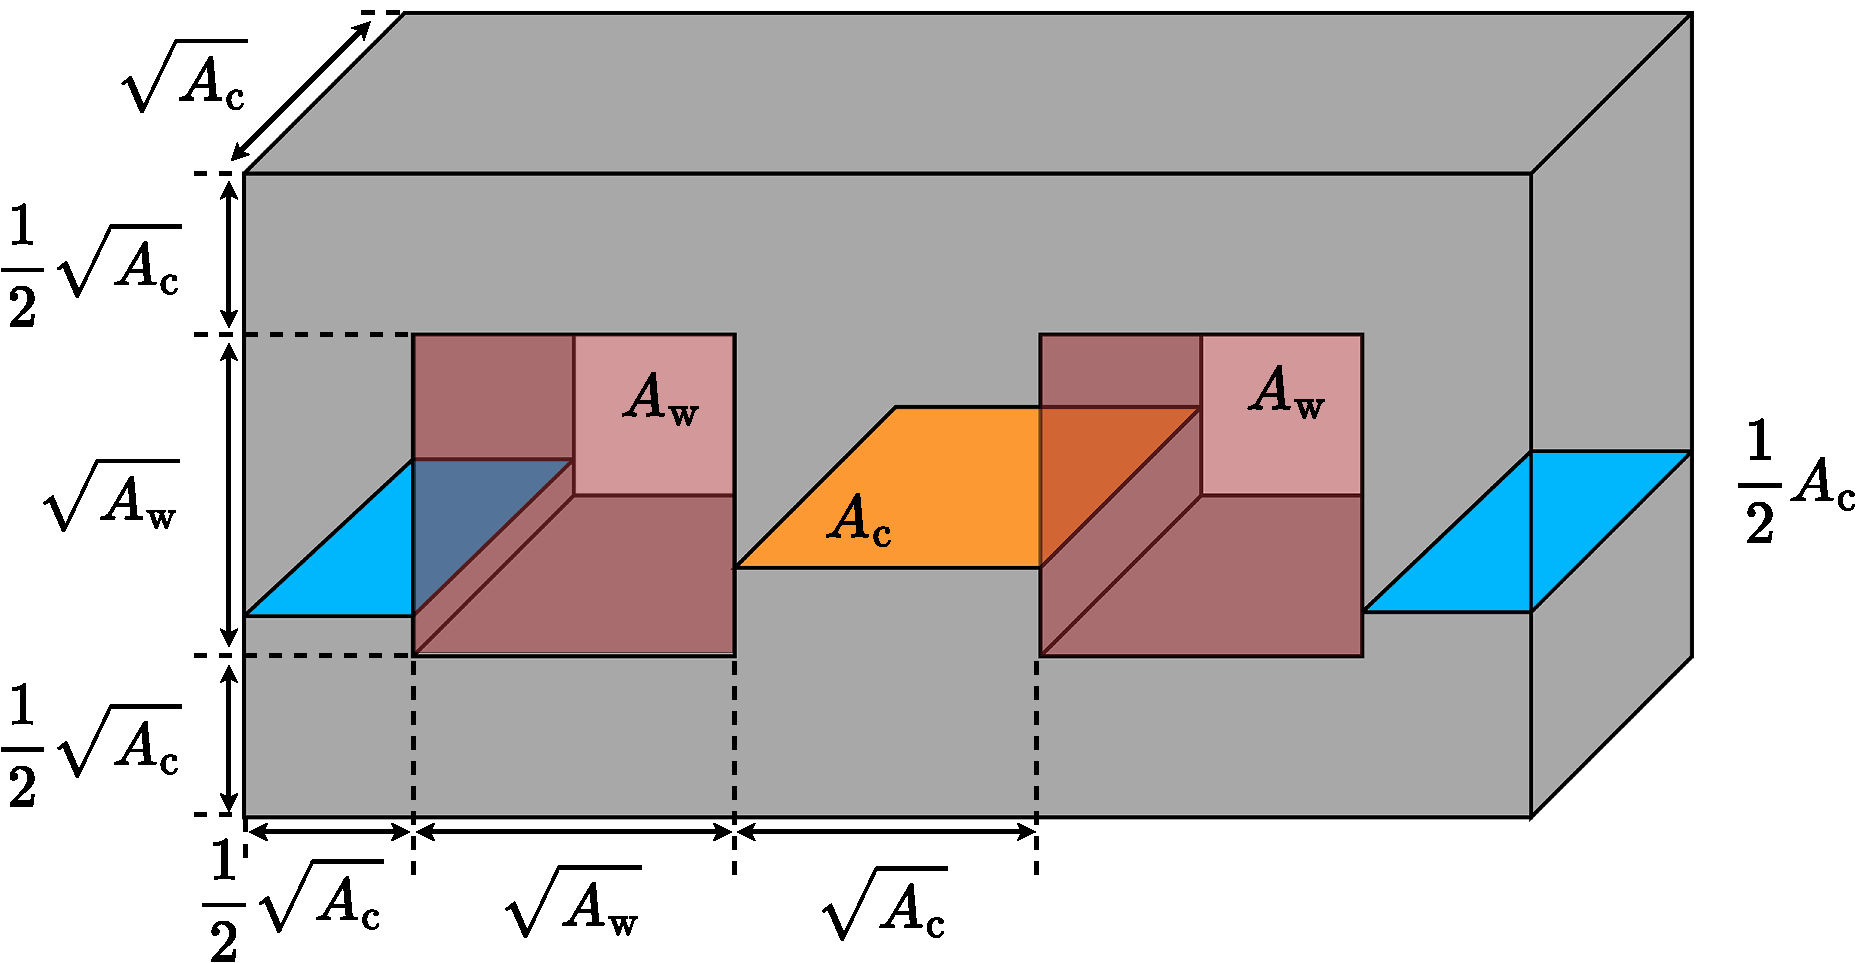
\includegraphics[width=\columnwidth]{Figures_v2/Fig14.pdf} % Make sure this file exists
        
        \caption{Simplified representation of one EE-core used in the volume analysis, with $A_c$ and $A_w$ redesigned to be square.}
        \label{fig:14}
\end{figure}


For the conventional transformer, $A_{\mathrm{c}}$ is expressed in \eqref{eq:28}. Here, $N_{\mathrm{p}}$ is the number of turns wound on the center leg of the conventional transformer.
\begin{equation}
\label{eq:28}
A_{\mathrm{c}_{\mathrm{conv}}} = \frac{L_{\mathrm{m}} I_{\mathrm{p}_{\mathrm{pk}}}}{B_{\mathrm{max}} N_{\mathrm{p}}}
\end{equation}
For the integrated transformer $A_{\mathrm{c}}$ is expressed in \eqref{eq:29}.
\begin{equation}
\label{eq:29}
A_{\mathrm{c}_{\mathrm{integ}}} = \frac{2 L_{\mathrm{m}} I_{\mathrm{p}_{\mathrm{pk}}}}{B_{\mathrm{max}} N_{12}} = \frac{L_{\mathrm{m}} I_{\mathrm{p}_{\mathrm{pk}}}}{B_{\mathrm{max}} N_{56}}
\end{equation}

The window area $A_{\mathrm{w}}$ can be expressed in terms of winding area and the occupancy ratio $K_{\mathrm{u}}$, as seen in \eqref{eq:30} for the conventional transformer:
\begin{equation}
\label{eq:30}
A_{\mathrm{w}_{\mathrm{conv}}} K_{\mathrm{u}} = N_{\mathrm{p}} \frac{I_{\mathrm{p}_{\mathrm{rms}}}}{J_{\mathrm{m}}} + N_{\mathrm{s}} \frac{I_{\mathrm{s}_{\mathrm{rms}}}}{J_{\mathrm{m}}}
\end{equation}
which simplifies to:
\begin{equation}
\label{eq:30b}
A_{\mathrm{w}_{\mathrm{conv}}} = \frac{N_{\mathrm{p}}}{J_{\mathrm{m}} K_{\mathrm{u}}} \left(I_{\mathrm{p}_{\mathrm{rms}}} + \frac{I_{\mathrm{s}_{\mathrm{rms}}}}{n}\right)
\end{equation}
For the integrated transformer, taking into account that the core window has half the total turns of the transformer $N_{12}$ and $N_{34}$, the $A_{\mathrm{w}}$ can be expressed as seen in \eqref{eq:32}.
\begin{align}
\label{eq:32}
A_{\mathrm{w}_{\mathrm{integ}}} K_{\mathrm{u}} &= \left(N_{56} \frac{I_{\mathrm{p}_{\mathrm{rms}}}}{J_{\mathrm{m}}} + N_{78} \frac{I_{\mathrm{s}_{\mathrm{rms}}}}{J_{\mathrm{m}}}\right) \nonumber \\
&\quad + \frac{1}{2}\left(N_{12} \frac{I_{\mathrm{p}_{\mathrm{rms}}}}{J_{\mathrm{m}}} + N_{34} \frac{I_{\mathrm{s}_{\mathrm{rms}}}}{J_{\mathrm{m}}}\right)
\end{align}

The total volume of the conventional transformer can be expressed using the expression shown in \eqref{eq:33}, where $x$ is a constant that denotes the ratio $A_{\mathrm{c}}/A_{\mathrm{w}}$. The total volume of the conventional transformer is twice the integrated transformer.
\begin{equation}
\label{eq:33}
\mathrm{Vol}_{\mathrm{conv}} = 2 AP^{3/4} (x^{3/4} + 2 x^{1/4} + x^{-1/4})
\end{equation}
The rms expressions of the primary and secondary side current are given in \eqref{eq:34} and \eqref{eq:35} \cite{ref8}.
\begin{align}
I_{\mathrm{p}_{\mathrm{rms}}} &= \frac{V_{\mathrm{in}_{\mathrm{max}}} D}{L_{\mathrm{m}} f_{\mathrm{s}}} \sqrt{\frac{D}{3}} \label{eq:34}\\
I_{\mathrm{s}_{\mathrm{rms}}} &= \frac{V_{\mathrm{in}_{\mathrm{max}}} D}{L_{\mathrm{m}} f_{\mathrm{s}}} \sqrt{\frac{5 n D^3}{9 \pi} \cdot \frac{V_{\mathrm{in}_{\mathrm{max}}}}{V_{\mathrm{o}}}} \label{eq:35}
\end{align}

Using these equations with the actual dimensions of the core used in the experimental verification, a 19\% volume reduction has been achieved by the proposed design, with the comparison shown in Table \ref{tab:volume}.

\begin{table}[htbp]
    \caption{Volume Analysis of the Conventional and Proposed Transformer using Core OP44721EC}
    \centering
    \footnotesize % Fixed font size for consistency
    \setlength{\tabcolsep}{4pt} % Adjust horizontal padding to fit column
    \begin{tabular}{cccc}
        \hline
        \textbf{Item} & \textbf{Symbol} & \textbf{Conventional} & \textbf{Integrated} \\
        \hline \hline
        Magnetizing inductance & $L_{\mathrm{m}}$ & 82.8 $\mu$H & 82.8 $\mu$H \\
        Turn ratio & $n$ & 3 & 3 \\
        Primary side peak current & $I_{\mathrm{pri}_{\mathrm{pk}}}$ & 8.02 A & 8.02 A \\
        Primary side rms current & $I_{\mathrm{pri}_{\mathrm{rms}}}$ & 2.25 A & 2.25 A \\
        Secondary side rms current & $I_{\mathrm{sec}_{\mathrm{rms}}}$ & 6.88 A & 6.88 A \\
        Saturation flux density & $B_{\mathrm{max}}$ & 0.3 T & 0.3 T \\
        Maximum current density & $J$ & 5 A/mm$^2$ & 5 A/mm$^2$ \\
        Occupancy ratio & $K_{\mathrm{u}}$ & 0.3 & 0.3 \\
        Area Product & $\mathrm{AP}$ & 6703.21 mm$^4$ & 13406.42 mm$^4$ \\
        Core Volume & $\mathrm{Vol}$ & 10313.57 mm$^3$ & 8672.64 mm$^3$ \\
        \hline
    \end{tabular}
    \label{tab:volume}
\end{table}

\section{Experimental Verification of Proposed Design}

\subsection{Prototype Evaluation Circuit and Prototype Transformer}
A prototype two-phase interleaved flyback rectifier, shown in Fig. \ref{fig:10a} operating in DCM was built to verify the operation of the integrated transformer. The prototype integrated transformer, shown in \ref{fig:10b}, was also designed using the proposed method. The specifications of the two-phase interleaved flyback rectifier and transformer are shown in Tables \ref{tab:prototype_rectifier} and \ref{tab:prototype_transformer} respectively. The coupling coefficient between the two flyback transformers $k_{N_{12}-N_{56}}$ is 0.0005, showing that the coupling was almost eliminated.



\subsection{Experimental Results}
Fig. \ref{fig:16a} shows the 100 W experimental waveforms at 4 ms/div from the two-phase interleaved flyback rectifier with the proposed transformer, demonstrating power factor correction. Fig. \ref{fig:16b} presents 2 $\mu$s/div waveforms. No current is induced in either switch except during the resonance between the leakage inductance and the parasitic capacitance of the switch. During the inactive period of the transformer, secondary diode side current is zero. Moreover, after $i_{\mathrm{S}_1}$ and $i_{\mathrm{S}_2}$ reached zero when $S_1$ and $S_2$ switched off, the currents remained at zero. Therefore, the two flyback converters operate independently without magnetic coupling interference. The same phenomenon was observed at 240 W two-phase drive, as shown in Fig. \ref{fig:16c}. Single-phase drive at lower power at 32.5 W is also feasible as shown in Fig. \ref{fig:16d}.

% --- TABLE VI: Rectifier Specifications ---
\begin{table}[h]
    \caption{Specifications of the Prototype Two-Phase Interleaved Flyback Rectifier}
    \centering
    \footnotesize
    \setlength{\tabcolsep}{3pt} % Slightly tighter spacing to handle long text
    \begin{tabular}{ccc}
        \hline
        \textbf{Item} & \textbf{Symbol} & \textbf{Value / Component} \\
        \hline \hline
        AC input voltage & $v_{\mathrm{in}}$ & 100-240 V \\
        Maximum rated power & $P_{\mathrm{out}}$ & 240 W \\
        Output voltage & $V_{\mathrm{out}}$ & 48 V \\
        Switching frequency & $f_{\mathrm{s}}$ & 100 kHz \\
        Bridge diode & $BD$ & CD-DF408S \\
        Input capacitor & $C_{\mathrm{in}}$ & 1 $\mu$F \\
        Switch & $S_1, S_2$ & STF15N80k5 \\
        Secondary diode & $D_1, D_2$ & STPSC30H12CWL \\
        Output capacitor & $C_{\mathrm{out}}$ & 2 x 1mF (parallel) \\
        Snubber capacitor & $C_{\mathrm{sn}1}, C_{\mathrm{sn}2}$ & 2.2 nF \\
        Snubber resistor & $R_{\mathrm{sn}1}, R_{\mathrm{sn}2}$ & 30 k$\Omega$ \\
        Snubber diode & $D_{\mathrm{sn}1}, D_{\mathrm{sn}2}$ & VS-E7MH0112-M3/1 \\
        \hline
    \end{tabular}
    \label{tab:prototype_rectifier}
\end{table}

% --- TABLE VII: Transformer Specifications ---
\begin{table}[h]
    \caption{Prototype Integrated Transformer Specifications}
    \centering
    \footnotesize
    \setlength{\tabcolsep}{4pt} 
    \begin{tabular}{ccc}
        \hline
        \textbf{Item} & \textbf{Symbol} & \textbf{Value} \\
        \hline \hline
        Magnetizing inductance (Target) & $L_{\mathrm{m}}$ & 82.8 $\mu$H \\
        Magnetizing inductance of $N_{12}$ & $L_{\mathrm{m}1}$ & 86.1 $\mu$H \\
        Magnetizing inductance of $N_{56}$ & $L_{\mathrm{m}2}$ & 75.1 $\mu$H \\
        Turn ratio & $n$ & 3 \\
        Magnetic core & - & OP44721EC \\
        \multirow{2}{*}{Number of turns} & $N_{12}:N_{34}$ & 24:8 \\
                                         & $N_{56}:N_{78}$ & 15:5 \\
        Center leg air gap & $l_{\mathrm{gc}}$ & 0.650 mm \\
        Outer leg air gap & $l_{\mathrm{go}}$ & 0.500 mm \\
        Coupling coefficient of $N_{12}, N_{34}$ & $k_{N_{12}-N_{34}}$ & 0.970 \\
        Coupling coefficient of $N_{56}, N_{78}$ & $k_{N_{56}-N_{78}}$ & 0.979 \\
        Coupling coefficient of $N_{12}, N_{56}$ & $k_{N_{12}-N_{56}}$ & 0.0005 \\
        \hline
    \end{tabular}
    \label{tab:prototype_transformer}
\end{table}

\begin{figure}[htbp]
\centering
% (a) Top circuit
        \subfloat[]{
        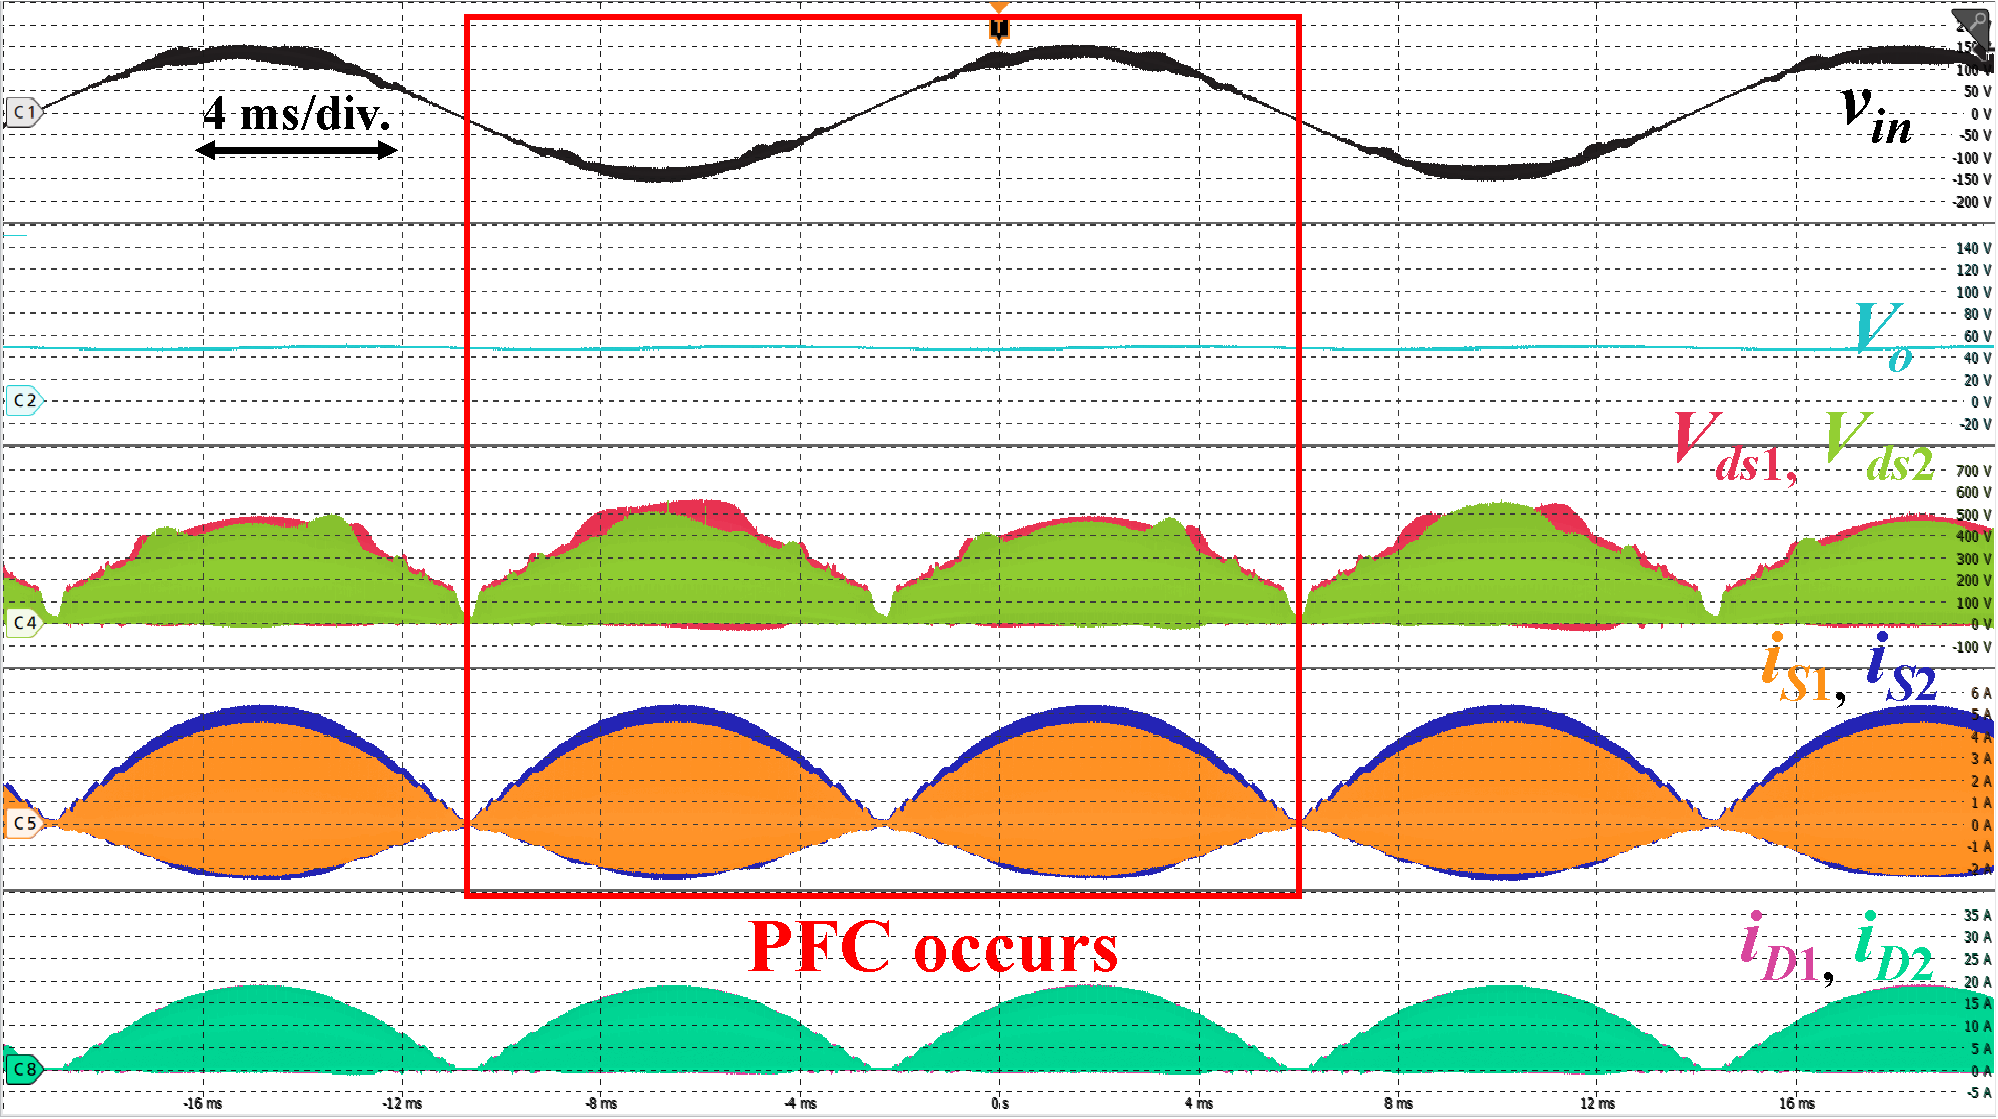
\includegraphics[width=0.9\columnwidth]{Figures_v2/Fig16a.pdf} % Make sure this file exists
        \label{fig:16a}}
        \\ % This double backslash forces the next image to the line below (vertical stack)
        % (b) Middle circuit
        \subfloat[]{
        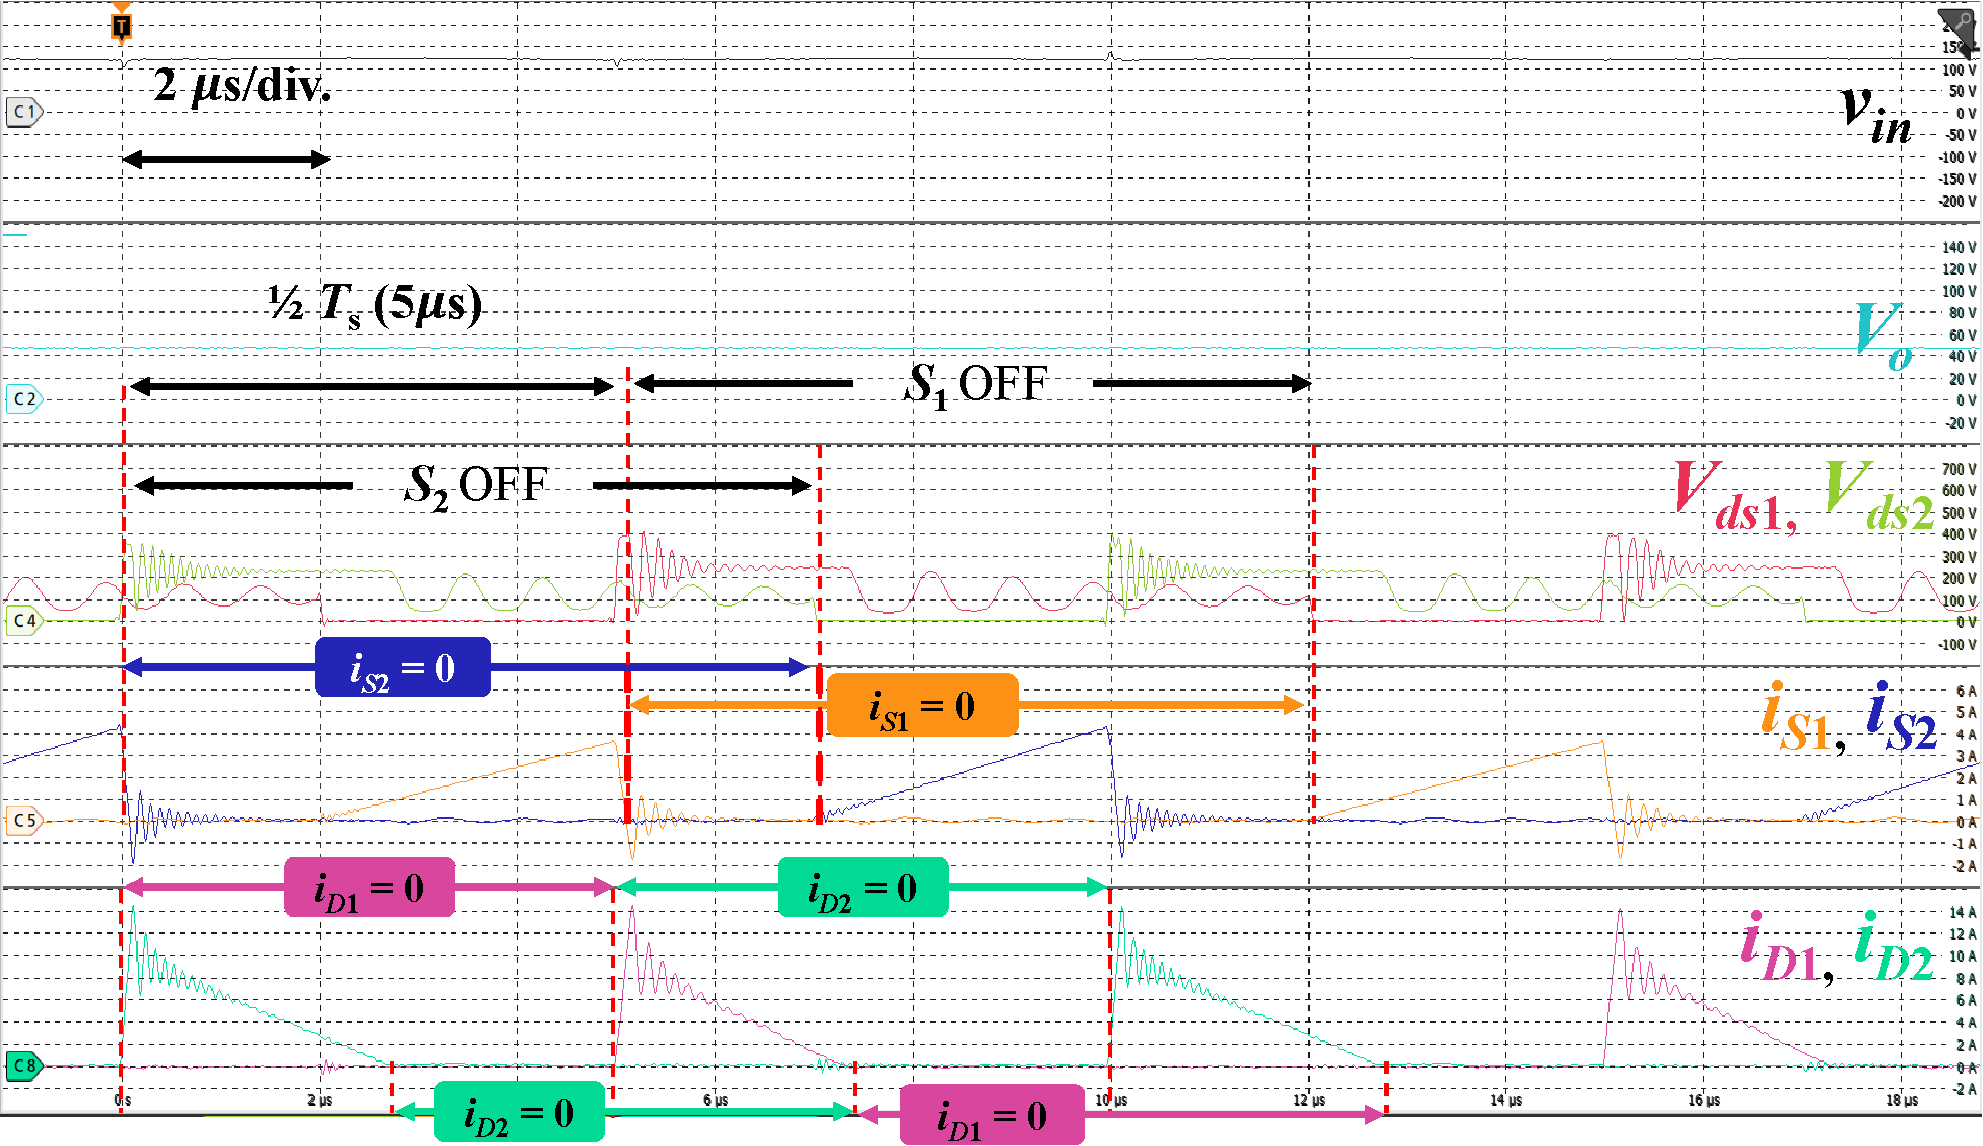
\includegraphics[width=0.9\columnwidth]{Figures_v2/Fig16b.pdf}
        \label{fig:16b}}
        \\ % This double backslash forces the next image to the line below (vertical stack)
        % (b) Middle circuit
        \subfloat[]{
        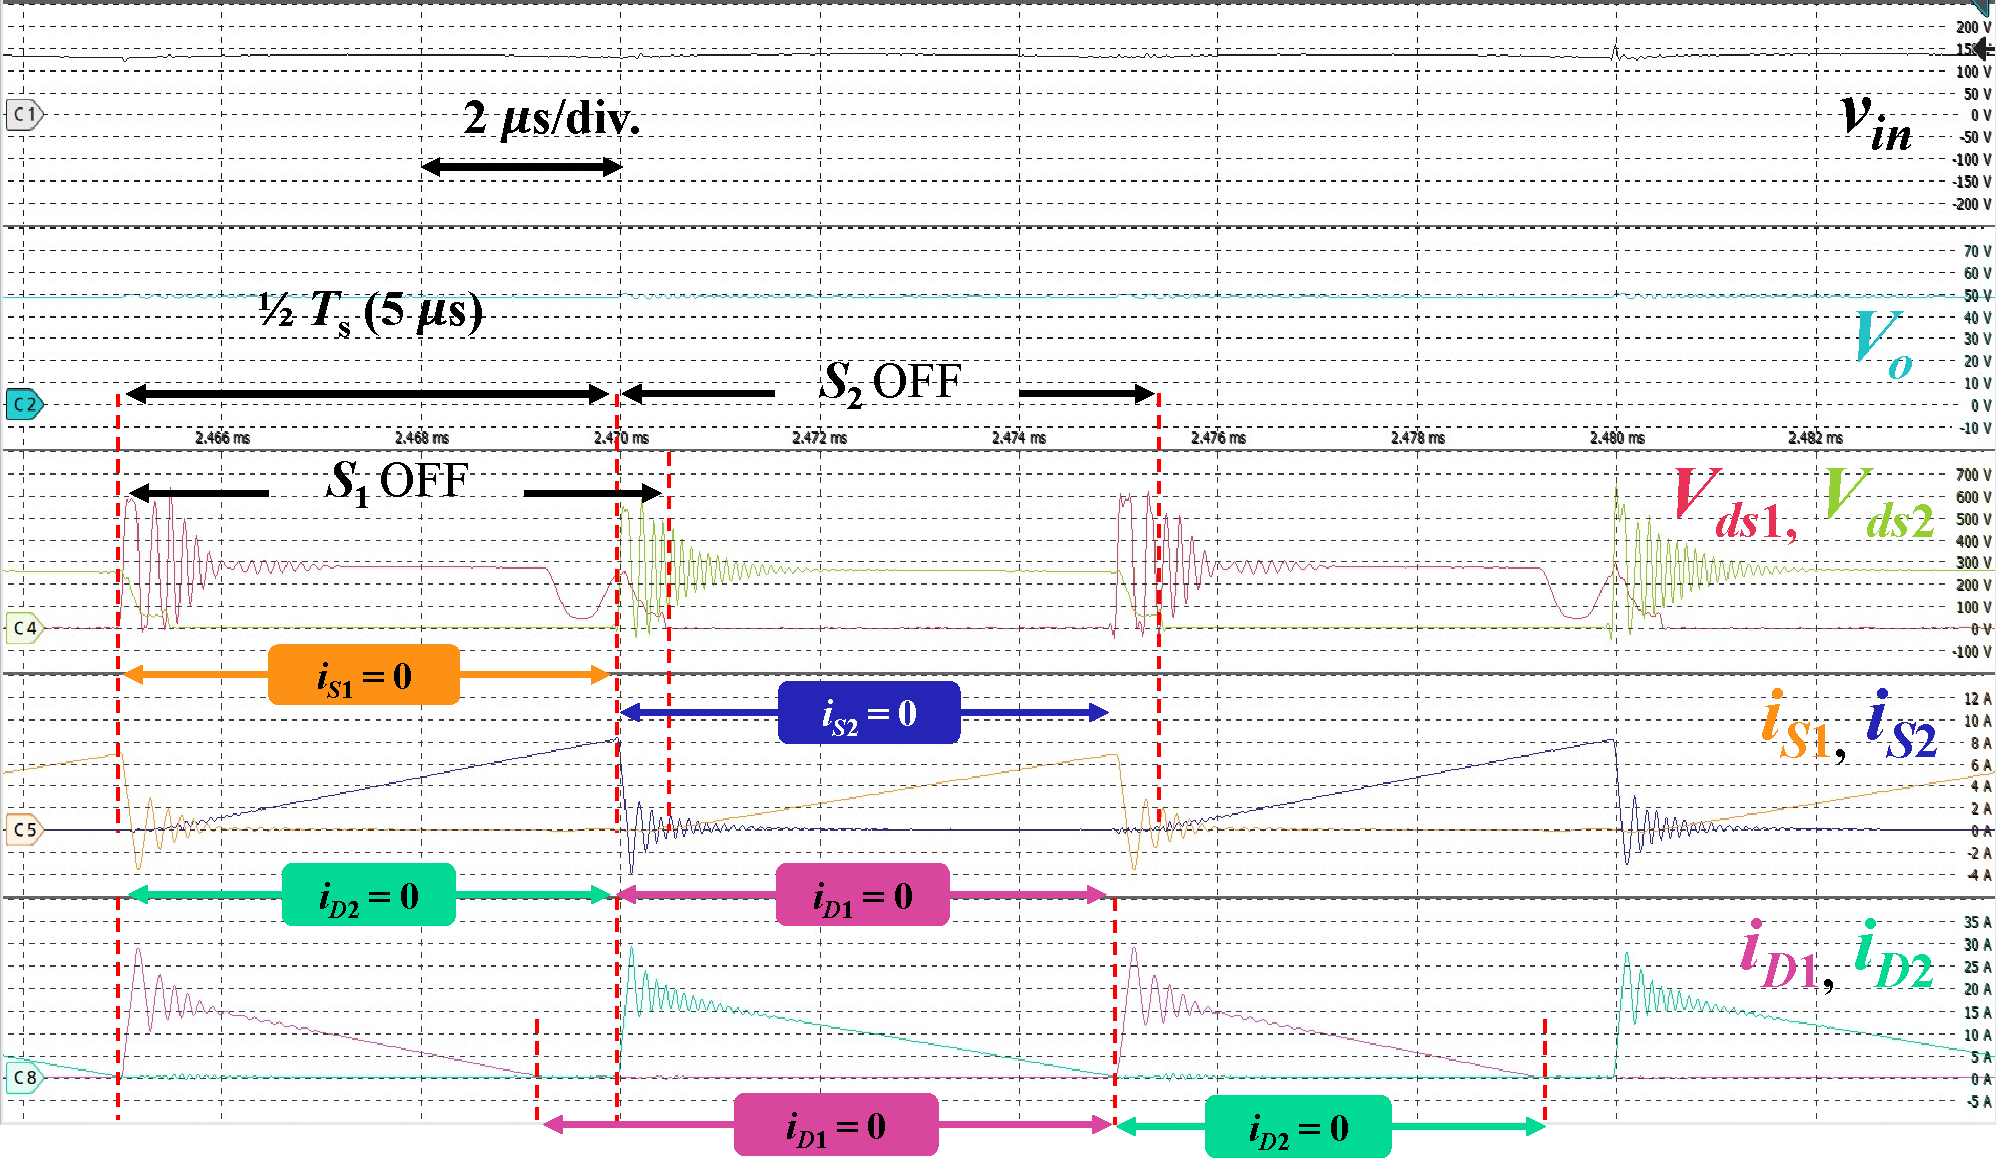
\includegraphics[width=0.9\columnwidth]{Figures_v2/Fig16c.pdf}
        \label{fig:16c}}
        \\ % This double backslash forces the next image to the line below (vertical stack)
        % (b) Middle circuit
        \subfloat[]{
        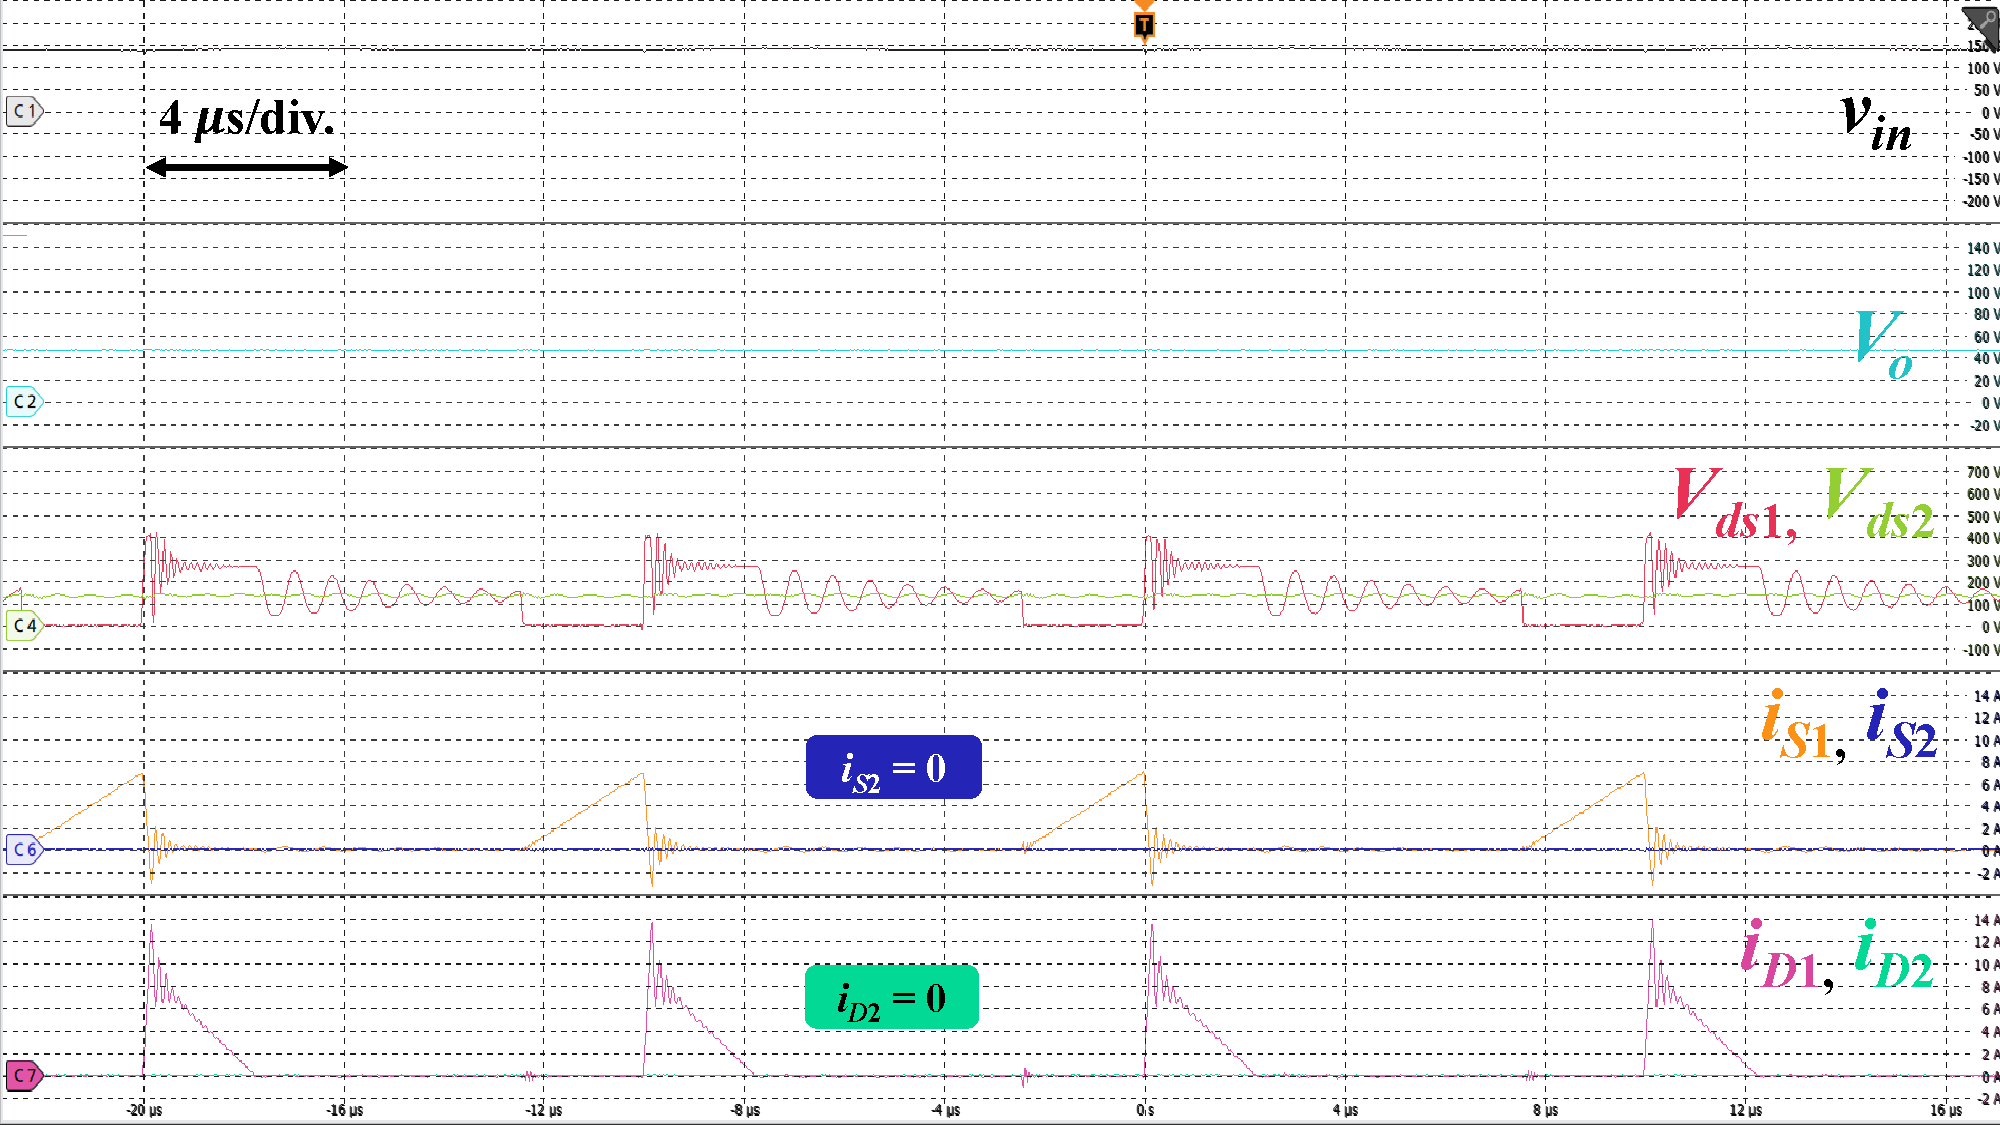
\includegraphics[width=0.9\columnwidth]{Figures_v2/Fig16d.pdf}
        \label{fig:16d}}
        
        \caption{Experimental waveforms of a two-phase interleaved flyback rectifier with the proposed integrated transformer at (a) \& (b): 100 W, two-phase AC drive, (c): 240 W, two-phase AC drive, (d): 32.5 W, single-phase AC drive. For (a) \& (b): $v_{\mathrm{in}}$: 50 V/div., $V_{\mathrm{o}}$: 10 V/div., $v_{\mathrm{ds}_1}, v_{\mathrm{ds}_2}$: 100 V/div., $i_{\mathrm{S}_1}, i_{\mathrm{S}_2}$: 1 A/div., $i_{\mathrm{D}_1}, i_{\mathrm{D}_2}$: 5 A/div.; For (c): $v_{\mathrm{in}}$: 50 V/div., $V_{\mathrm{o}}$: 10 V/div., $v_{\mathrm{ds}1}, v_{\mathrm{ds}2}$: 100 V/div., $i_{\mathrm{S}_1}, i_{\mathrm{S}_2}$: 2 A/div., $i_{\mathrm{D}_1}, i_{\mathrm{D}_2}$: 5 A/div.; For (d): $v_{\mathrm{in}}$: 50 V/div., $V_{\mathrm{o}}$: 20 V/div., $v_{\mathrm{ds}_1}, v_{\mathrm{ds}_2}$: 100 V/div., $i_{\mathrm{S}_1}, i_{\mathrm{S}_2}$: 2 A/div., $i_{\mathrm{D}_1}, i_{\mathrm{D}_2}$: 2 A/div.}
        \label{fig:16}
\end{figure}

\section{Conclusion}
In this paper, an integrated transformer was successfully designed for a two-phase interleaved flyback rectifier for USB PD 3.1 applications. The proposed winding structure for the integrated transformer prevents coupling between the two flyback transformers. A coupling coefficient of 0.0005 was achieved with the prototype. Independent flyback circuit operation without magnetic interference due to coupling was verified through simulation and experiment up to 240 W. Because of the proposed design, two transformers are integrated into one component, enabling the downsizing of magnetic components by about 19\% compared to the conventional transformer.

% --- TABLE V: Volume Analysis ---




% --- TABLE VII: Transformer Specifications ---
% --- TABLE VII: Transformer Specifications ---


\begin{thebibliography}{1}
\bibliographystyle{IEEEtran}

\bibitem{ref1}
A. Medina-Garcia, J. Cruz-Cozar, D. P. Morales-Santos, N. Rodriguez, and M. Schlenk, "A High-Efficiency Isolated Wide Voltage Range DC-DC Converter Using WBG Devices," \textit{IEEE Access}, vol. 10, pp. 84818-84825, Aug. 2022.

\bibitem{ref2}
USB-IF PR, "USB Promoter Group Announces USB Power Delivery Specification Revision 3.1," 2021. [Online]. Available: https://www.usb.org/sites/default/files/2021-05/USB\%20PG\%20USB\%20PD\%203.1\%20DevUpdate\%20Announcement\_FINAL.pdf

\bibitem{ref3}
B. C. Kim, K. B. Park, C. E. Kim, B. H. Lee, and G. W. Moon, "LLC resonant converter with adaptive link-voltage variation for a high-power-density adapter," \textit{IEEE Trans. Power Electron.}, vol. 25, no. 9, pp. 2248-2252, May 2010.

\bibitem{ref4}
Y. C. Lin, F. C. Lee, Q. Li, X. Huang, and Z. Lin, "A novel AC-to-DC adaptor with ultra-high power density and efficiency," in \textit{IEEE Applied Power Electronics Conference and Exposition}, 2016, pp. 1853-1860.

\bibitem{ref5}
M. Li, Z. Ouyang, and M. A. E. Andersen, "Analysis and optimal design of high-frequency and high-efficiency asymmetrical half-bridge flyback converters," \textit{IEEE Trans. Indus. Electron.}, Vol. 67, no. 10, pp. 8312-8321, Nov. 2019.

\bibitem{ref6}
X. Huang, J. Feng, W. Du, F. C. Lee, and Q. Li, "Design consideration of MHz active clamp flyback converter with GaN devices for low power adapter application," in \textit{2016 IEEE Applied Power Electronics Conference and Exposition (APEC)}, 2016, pp. 2334-2341.

\bibitem{ref7}
J. Zhang, X. Huang, X. Wu, and Z. Qian, "A high efficiency flyback converter with new active clamp technique," \textit{IEEE Trans. Power Electron.}, vol. 25, no. 7, pp. 1775-1785, Feb. 2010.

\bibitem{ref8}
J. Shin, S. Choi and B. Cho, "High-efficiency bridgeless flyback rectifier with bidirectional switch and dual output windings," \textit{IEEE Trans. Power Electron.}, vol. 29, no. 9, pp. 4752-4762, Oct. 2013.

\bibitem{ref9}
S. Choi, J. Shin, J. Imaoka and M. Yamamoto, "Common-Mode Noise Reduction of Bridgeless Flyback PFC Rectifier with Balance Technique," \textit{IEICE Tech Rep}, vol. 123, no. 119, pp. 67-72, 2023.

\bibitem{ref10}
K. T. Mok, Y. M. Lai, and K. H. Loo, "A single-stage bridgeless power-factor-correction rectifier based on flyback topology," in \textit{2011 IEEE 33rd International Telecommunications Energy Conference (INTELEC)}, 2011, pp. 1-6.

\bibitem{ref11}
J. Beak, J. Shin, P. Jang, and B. Cho, "A critical conduction mode bridgeless flyback converter," \textit{8th International Conference on Power Electronics-ECCE Asia}, 2011, pp. 487-492.

\bibitem{ref12}
B. Shafer, "Interleaving contributes unique benefits to forward converters and flyback converters," in \textit{Texas Instrument Power Supply Design Seminar}, Topic, vol. 4, pp. 1-32, 2004.

\bibitem{ref13}
L. P. Wong, Y. S. Lee, and D. K. W. Cheng, "A new approach to the analysis and design of integrated magnetics," in \textit{Sixteenth IEEE Applied Power Electronics Conference and Exposition}, 2001, pp. 1196-1202.

\bibitem{ref14}
S. Choi, J. Shin, J. Imaoka, and M. Yamamoto, "Voltage-Controlled Variable Inductor for Fixed-Frequency Critical Conduction Mode Operation," \textit{IEEE Trans. Indus. Electron}, vol. 70, no. 6, pp. 5707-5716, Aug. 2022.

\bibitem{ref15}
M. Ishihara, S. Kimura, W. Martinez and M. Yamamoto, "Analysis and design of passive components for interleaved flyback converter with integrated transformer," in \textit{2015 IEEE Energy Conversion Congress and Exposition (ECCE)}, 2015, pp. 5902-5909.

\bibitem{ref16}
M. Taheri, J. Milimonfared, H. Bayat, H. Riazmontazer and A. Noroozi, "Analysis and design of a new soft switching interleaved converter using an integrated transformer," in \textit{2011 2nd Power Electronics, Drive Systems and Technologies Conference}, 2011, pp. 98-103.

\bibitem{ref17}
T. Qian and B. Lehman, "Coupled Input-Series and Output-Parallel Dual Interleaved Flyback Converter for High Input Voltage Application," \textit{IEEE Trans. Power Electron.}, vol. 23, no. 1, pp. 88-95.

\bibitem{ref18}
Liang Yan, Dayu Qu and B. Lehman, "Integrated magnetic full wave converter with flexible output inductor," in \textit{Seventeenth Annual IEEE Applied Power Electronics Conference and Exposition}, 2002, pp. 824-830.

\bibitem{ref19}
G. B. Koo, "Design guidelines for RCD snubber of flyback converters," Fairchild Semiconductor, San Jose, CA, USA, Appl. Note AN-4147 Rev. 1.1.0, 2006.

\bibitem{ref20}
W. McMurray, "Selection of snubbers and clamps to optimize the design of transistor switching converters," \textit{IEEE Transactions on Industry Applications}, vol. IA-16, no. 4, pp. 513-523, 1980.

\bibitem{ref21}
W. Colonel and T. McLyman, \textit{Transformer and Inductor Design Handbook}. Boca Raton, FL, USA: CRC Press, 2004.

\bibitem{ref22}
S. Kimura, S. Aoto, M. Ishihara, J. Imaoka and M. Yamamoto, "Interleaved active clamp forward converter with novel integrated magnetic components," in \textit{2015 IEEE Energy Conversion Congress and Exposition (ECCE)}, 2015, pp. 6029-6036.

\end{thebibliography}

%\begin{IEEEbiography}[{\includegraphics[width=1in,height=1.25in,clip,keepaspectratio]{karl_photo}}]{Karl Raymond Dela Cruz Roque}
%(Student Member, IEEE) is with the Graduate School of Engineering, Nagoya University, Nagoya, 464-8601, Japan.
%\end{IEEEbiography}
%
% Placeholder for other biographies if needed
\vfill

\end{document}